% Este documento tem a ver com as partes do LIVRO. 

\thispagestyle{empty}

\begin{textblock*}{-2in}(0pt,0pt)%
\vspace*{-1.8cm}
\hspace*{-3cm}
\includegraphics[width=142mm]{./ABERTURA.png}  
\end{textblock*}

\pagebreak
\blankpage

%\blankpage

% Tamanhos
% \tiny
% \scriptsize
% \footnotesize
% \small 
% \normalsize
% \large 
% \Large 
% \LARGE 
% \huge
% \Huge

% Posicionamento
% \centering 
% \raggedright
% \raggedleft
% \vfill 
% \hfill 
% \vspace{Xcm}   % Colocar * caso esteja no começo de uma página. Ex: \vspace*{...}
% \hspace{Xcm}

% Estilo de página
% \thispagestyle{<<nosso>>}
% \thispagestyle{empty}
% \thispagestyle{plain}  (só número, sem cabeço)
% https://www.overleaf.com/learn/latex/Headers_and_footers

% Compilador que permite usar fonte de sistema: xelatex, lualatex
% Compilador que não permite usar fonte de sistema: latex, pdflatex

% Definindo fontes
% \setmainfont{Times New Roman}  % Todo o texto
% \newfontfamily\avenir{Avenir}  % Contexto
\begingroup\thispagestyle{empty}\vspace*{.05\textheight} 

              \formular
              \huge
              \noindent
              \textbf{A mulher que\\virou tatu}
              
              \vspace{0.3em}

              \noindent\Large\textit{Yuxabu yaixni}
                    
\endgroup
\vfill
\pagebreak       % [Frontistício]
%\newcommand{\linhalayout}[2]{{\tiny\textbf{#1}\quad#2\par}}
\newcommand{\linha}[2]{\ifdef{#2}{\linhalayout{#1}{#2}}{}}

\begingroup\tiny
\parindent=0cm
\thispagestyle{empty}

\textbf{edição brasileira©}\quad			 {Hedra \the\year}\\
\textbf{organização}\quad		 			 {Eliane Camargo}\\
%\textbf{tradução}\quad			 			 {Izaque João}\\
%\textbf{posfácio©}\quad			 		 {Fábio Zuker}\\
\textbf{ilustração©}\quad			 		 {Anita Ekman}\medskip

\textbf{edição consultada}\quad			 {Transcrição feita por Capistrano de Abreu}\\
%\textbf{primeira edição}\quad			 	 {Acontecimentos}\\
%\textbf{agradecimentos}\quad			 	 {agradecimentos}\\
%\textbf{indicação}\quad			 		 {indicacao}\medskip

\textbf{coordenação da coleção}\quad		 {Luísa Valentini}\\
\textbf{edição}\quad			 			 {Jorge Sallum}\\
\textbf{coedição}\quad			 			 {Suzana Salama}\\
\textbf{assistência editorial}\quad			 {Paulo Henrique Pompermaier}\\
\textbf{revisão}\quad						 {Renier Silva}\\				
\textbf{capa}\quad			 				 {Lucas Kroëff}\\
%\textbf{iconografia}\quad			 		 {iconografia}\\
%\textbf{imagem da capa}\quad			 	 {imagemcapa}\medskip

\textbf{\textsc{isbn}}\quad			 		 {978-65-89705-72-7}

\hspace{-5pt}\begin{tabular}{ll}
\textbf{conselho editorial} & Adriano Scatolin,  \\
							& Antonio Valverde,  \\
							& Caio Gagliardi,    \\
							& Jorge Sallum,      \\
							& Ricardo Valle,     \\
							& Tales Ab'Saber,    \\
							& Tâmis Parron      
\end{tabular}
 
\bigskip
\textit{Grafia atualizada segundo o Acordo Ortográfico da Língua\\
Portuguesa de 1990, em vigor no Brasil desde 2009.}\\

\vfill
\textit{Direitos reservados em língua\\ 
portuguesa somente para o Brasil}\\

\textsc{editora hedra ltda.}\\
R.~Fradique Coutinho, 1139 (subsolo)\\
05416--011 São Paulo \textsc{sp} Brasil\\
Telefone/Fax +55 11 3097 8304\\\smallskip
editora@hedra.com.br\\
www.hedra.com.br\\

Foi feito o depósito legal.

\endgroup
\pagebreak     % [Créditos]
% Tamanhos
% \tiny
% \scriptsize
% \footnotesize
% \small 
% \normalsize
% \large 
% \Large 
% \LARGE 
% \huge
% \Huge

% Posicionamento
% \centering 
% \raggedright
% \raggedleft
% \vfill 
% \hfill 
% \vspace{Xcm}   % Colocar * caso esteja no começo de uma página. Ex: \vspace*{...}
% \hspace{Xcm}

% Estilo de página
% \thispagestyle{<<nosso>>}
% \thispagestyle{empty}
% \thispagestyle{plain}  (só número, sem cabeço)
% https://www.overleaf.com/learn/latex/Headers_and_footers

% Compilador que permite usar fonte de sistema: xelatex, lualatex
% Compilador que não permite usar fonte de sistema: latex, pdflatex

% Definindo fontes
% \setmainfont{Times New Roman}  % Todo o texto
% \newfontfamily\avenir{Avenir}  % Contexto

\begingroup\thispagestyle{empty}\vspace*{.05\textheight} 

              \formular
              \huge
              \noindent
              \textbf{A mulher que virou tatu}

              \bigskip  
              
              \large
              \noindent
              \textit{Yuxabu yaixni}
              \vspace{12.5em}
              
              \newfontfamily\garamond{EBGaramond12-Regular}
              {\selectfont\garamond\small\noindent Eliane camargo (\textit{organização})}

              {\selectfont\garamond\small\noindent Anita Ekman (\textit{ilustração})}

              {\selectfont\garamond\small\noindent Capistrano de Abreu (\textit{transcrição})}

              \bigskip

              \noindent
              {\selectfont\garamond\small\noindent 2ª edição}

              \vfill

              \newfontfamily\timesnewroman{Times New Roman}
              {\noindent\fontsize{30}{40}\selectfont \timesnewroman hedra}

              \noindent{\selectfont\garamond\small
              \noindent São Paulo \quad\the\year}


\endgroup
\pagebreak
	       % [folha de rosto]
% nothing			is level -3
% \book				is level -2
% \part				is level -1
% \chapter 			is level 0
% \section 			is level 1
% \subsection 		is level 2
% \subsubsection 	is level 3
% \paragraph 		is level 4
% \subparagraph 	is level 5
\setcounter{secnumdepth}{-2}
\setcounter{tocdepth}{0}

% \renewcommand{\contentsname}{Índex} 	% Trocar nome do sumário para 'Índex'
%\ifodd\thepage\relax\else\blankpage\fi 	% Verifica se página é par e coloca página branca
%\tableofcontents*

\pagebreak
\begingroup \footnotesize \parindent0pt \parskip 5pt \thispagestyle{empty} \vspace*{-0.5\textheight}\mbox{} \vfill
\baselineskip=.92\baselineskip
\textbf{A mulher que virou tatu} \textls[10]{é uma história originalmente registrada no início do século \textsc{xx}, pelo historiador João Capistrano de Abreu. A língua hoje não é mais escrita do modo como Capistrano a registrou, portanto esta edição é atualizada --- além de bilíngue e ilustrada. Fala de dois alimentos que os Caxinauá plantam: o milho, mais apreciado e de cultivo mais difícil, e a batata doce, mais rápido e simples. Na história, a família de uma velha lhe dá batata doce por dar menos trabalho de produzir, já que os idosos Caxinauá não trabalham e sua alimentação deve ser garantida pelos parentes.}

\textbf{Eliane Camargo} é etnolinguista. É doutora em Linguística Descritiva pela Universidade de Paris (Sorbonne) e estuda a língua e cultura de três grupos indígenas, os Caxinauá, os Aparai e os Wayana. Coordenou, entre 2006 e 2011, a divisão etnolinguística do projeto de documentação franco-alemão da cultura e língua Caxinauá do \textsc{dobes}.

\textbf{Anita Ekman} é artista visual, \textit{performer} e ilustradora que trabalha com as artes ameríndias e afro-brasileiras. Como especialista em arte indígena, trabalhou na formação da coleção \textit{Great Masters of Popular Art in Ibero-America}, do Banamex Cultural Fund.

\textbf{Capistrano de Abreu} \textls[20]{(1953--1927) foi historiador, mas produziu também dentro dos campos da etnografia e linguística. Em 1914 registrou, pela primeira vez, a língua e o modo de vida Caxinauá junto a dois jovens provenientes do povo, do rio Ibuaçu. Esse trabalho deu origem ao livro \textit{Hantxa huni kuin}, sobre a língua dos Caxinauá do rio Ibuaçu, afluente do Muru.}

\pagebreak
\thispagestyle{empty}

\textls[-5]{\textbf{Mundo Indígena} reúne materiais produzidos com pensadores de diferentes povos indígenas e pessoas que pesquisam, trabalham ou lutam pela garantia de seus direitos. Os livros foram feitos para serem utilizados pelas comunidades envolvidas na sua produção, e por isso uma parte significativa das obras é bilíngue. Esperamos divulgar a imensa diversidade linguística dos povos indígenas no Brasil, que compreende mais de 150 línguas pertencentes a mais de trinta famílias linguísticas.}\looseness=-1



\endgroup

\pagebreak\thispagestyle{empty}\movetooddpage
{\begingroup\mbox{}\pagestyle{empty}
\pagestyle{empty} 
% \renewcommand{\contentsname}{Índex} 	% Trocar nome do sumário para 'Índex'
%\ifodd\thepage\relax\else\blankpage\fi 	% Verifica se página é par e coloca página branca
\addtocontents{toc}{\protect\thispagestyle{empty}}
\tableofcontents*\clearpage\endgroup}

\chapter{Nota da organizadora}

\textls[10]{Esta história fala de dois alimentos que os Caxinauá cultivam em seus roçados, o milho e a batata doce. A batata doce é uma raiz tuberosa e de fácil cultivo: plantando uma só vez é possível colher muitas vezes, pela propagação de suas ramas. Já o cultivo do milho é mais trabalhoso: a cada vez que se colhe, é preciso esperar a época de plantio para plantar as sementes, que leva cerca de seis meses para colher novamente. Os Caxinauá apreciam e consomem mais o milho, mas também plantam a batata doce, por crescer rápido e dar pouco trabalho.}

Os idosos caxinauá não trabalham no roçado; sua alimentação deve ser garantida pelos seus genros e por sua família em geral. Na história, a família da velha lhe dá batata doce
por dar menos trabalho de produzir.

\textls[-10]{Ao comer o milho verde, que é mais macio, a família, sobretudo o genro, reclama por ela não deixar o milho amadurecer, o que a deixa triste e a leva a querer virar tatu.}

\section{quem são os caxinauá}

\textls[20]{A família linguística pano é composta por cerca de trinta grupos, espalhados em uma vasta região transfronteiriça entre a Bolívia, o Brasil e o Peru.}

Os quase oito mil Caxinauá fazem parte desta família, ocupando a fronteira entre o Brasil
e o Peru. No Brasil, eles vivem em 12 terras indígenas e, no Peru, eles ocupam todo o rio Curanja e uma parte do rio Purus --- da cidade de Puerto Esperanza até a embocadura
do rio Curanja.

\textls[20]{No Peru, e na região do rio Purus, no Peru e no Brasil, as mulheres e crianças falam apenas a língua caxinauá. Nas demais regiões elas já são bilíngues e, em alguns locais,
monolíngues em português.}

\textls[20]{Todas as comunidades têm escola formal, onde são somente alfabetizados em caxinauá. O
restante do ensino é ministrado em espanhol, no Peru, e em português, no Brasil. O material escolar em língua caxinauá é escasso no Peru, e corrente no Brasil.}
\chapter{Como foi feito este livro}

No início do século \textsc{xx}, o historiador João Capistrano de Abreu trabalhou
com dois jovens caxinauás provenientes do rio Ibuaçu, afluente do rio Muru, por sua vez afluente do rio Tarauacá, na bacia do rio Juruá, no estado do Acre.

Com a venda de borracha de sua região, estes jovens foram levados para Manaus. Lá eles conheceram Luís Sombra, amigo de Capistrano de Abreu, que os encaminhou ao historiador, cada um de uma vez, para o Rio de Janeiro, onde ficaram na casa de Capistrano e trabalharam
com ele no registro da sua língua e de seu modo de vida.

Esse trabalho deu origem ao livro \textit{Hantxa huni kuin, a língua dos caxinauás do rio Ibuaçu, afluente do muru} (prefeitura de Tarauacá). O livro foi publicado pela primeira vez em 1914.

Hoje em dia, a língua caxinauá não é escrita do modo que Capistrano a
registrou, e os próprios caxinauá não conseguem ler esses relatos de
cem anos atrás. Além disso, a língua ainda não era muito estudada, então
a tradução proposta por Capistrano era muito entrecortada e inicial.


\textls[-20]{Pensando que essas histórias poderiam ser lidas hoje em uma forma mais acessível tanto aos caxinauá quanto aos falantes de português, a linguista Eliane Camargo, que
trabalha com eles desde 1987, resolveu revisar o livro e refazer a tradução, dentro do programa de documentação de cultura e língua caxinauá, \textsc{dobes}, financiado pela
Fundação Volkswagen.}\looseness=-1

Esta história é uma parte dessa versão revisada por Eliane, que consideramos ser interessante para crianças e para adultos e, por isso, publicamos neste livrinho. Uma parte
dos direitos autorais recebidos com a publicação do livro será destinada à realização de oficinas de língua e cultura onde os caxinauá continuarão pensando novos modos de
escrever e apresentar sua língua e sua cultura em suas próprias escolas e para pessoas de outros lugares.



\chapter[Para ler as palavras caxinauá]{Para ler as palavras\break caxinauá}

A língua caxinauá apresenta quatro vogais --- \textit{a}, \textit{e}, \textit{i}, \textit{u} --- e catorze consoantes --- \textit{b}, \textit{d}, \textit{h}, \textit{k}, \textit{m}, \textit{n}, \textit{p}, \textit{s}, \textit{x}, \textit{t}, \textit{ts}, \textit{tx}, \textit{w}, \textit{y}. Notem que \textit{a} ordem do \textit{x} na sequência do alfabeto muda;
ele aparece logo após o \textit{s}.

Nesta língua há três sons não existentes em português:

\begin{itemize}
\item A vogal \textit{e} que é um \textit{schwa}, ou seja, um \textit{e} pronunciado com \textit{a} língua plana e o som sai de trás. Este som é comum em inglês, em francês e em muitas línguas da amazônia;

\item A consoante \textit{ts} requer uma pronuncia em um só som, \textit{t}\,+\,\textit{s};

\item A consoante \textit{x} é uma retroflexa, isto é, a massa da língua vai para trás e a ponta dela toca ligeiramente o palato. Este som é comum em chinês;

\item Sequência consonântica \textit{t}\,+\,\textit{x} (\textit{tch}) é comum em espanhol, grafado \textit{ch}.
\end{itemize}

As palavras dissilábicas são muito comuns:

\begin{itemize}
\item Baka, como em \textit{peixe};
\item Hiwe, como em \textit{casa};
\item Kene, como em \textit{grafismo};
\item Tapu, como em \textit{jirau}, \textit{ponte}.
\end{itemize}

Mas há palavras de uma só sílaba: \textit{hi}, ``árvore''; ou de mais sílabas: \textit{taka}--da, ``galinha''; \textit{bepukudu}, ``borboleta''.



\openany\raggedright

\blankpage
\part[A mulher que virou tatu]{A mulher que\\ virou tatu}

\chapter*{}

\mbox{}\vspace*{\fill}

% \begin{verse}
% \letra{Q}{uando} a família se reunia, só se comia\\
% batata doce. Faziam roçado e plantavam\\
% batata doce. Só davam batata doce bichada\\
% para a velha comer. É o que davam à velha.\\
% Ela vivia com a família.
% \end{verse}

\begingroup\setlength{\linewidth}{.6\linewidth}

\letra{Q}{uando} a família se reunia, só se comia
batata doce. Faziam roçado e plantavam
batata doce. Só davam batata doce bichada
para a velha comer. É o que davam à velha.
Ela vivia com a família.

\vspace{2em}

% \begin{verse}
% \textit{Kadi besti pikin, itxa wani kiaki.\\
% Bai wakin hawen ni katsidan, kadi banaaki.\\
% Xena besti pimiski hawen pitimaken.\\
% Yuxabudan eskani kiaki.Hawen\\
% nabube hiwea.}
% \end{verse}

\letra{K}{adi} besti pikin, itxa wani kiaki.
Bai wakin hawen ni katsidan, kadi banaaki.
Xena besti pimiski hawen pitimaken.
Yuxabudan eskani kiaki.Hawen
nabube hiwea.

\vspace*{\fill}

\pagebreak
\thispagestyle{empty}
\begin{figure}
\vspace*{-.5cm}
\hspace*{-2.3cm}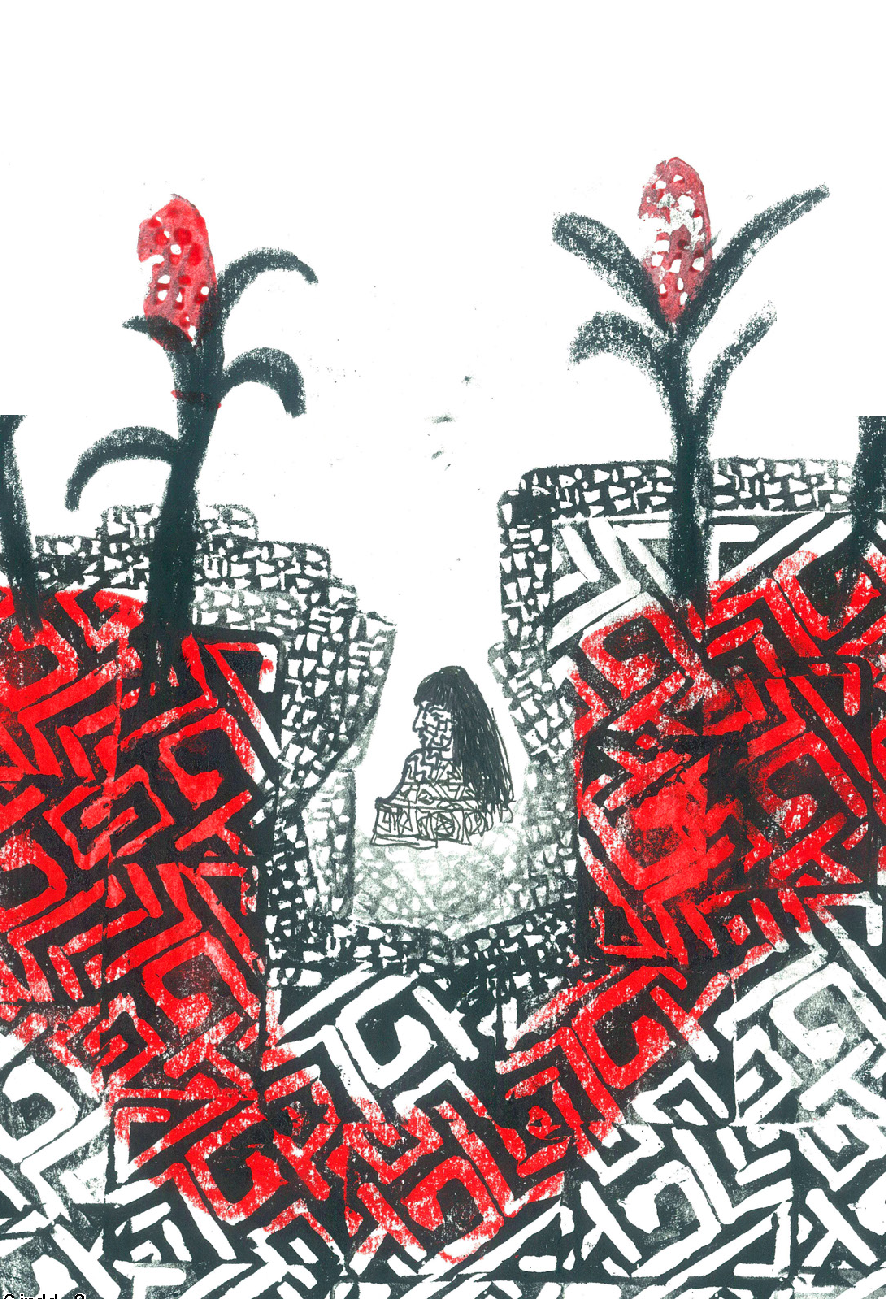
\includegraphics[width=140mm]{./imgs/img1.pdf}
\end{figure}

\chapter*{}

\mbox{}\vspace*{\fill}

% \begin{verse}
% A família dela fazia roçado e tinha\\
% um milharal. A velha desdentada\\
% não podia comer milho seco.
% \end{verse}

% \begin{verse}
% \textit{Hawen nabu bai waxun, xeki\\
% banaimabu. Yuxabudan xeta uma,\\
% haska waxun piti, kuxi pitima.}
% \end{verse}


\letra{A}{família} dela fazia roçado e tinha
um milharal. A velha desdentada
não podia comer milho seco.

\vspace{2em}

\letra{H}{awen} nabu bai waxun, xeki
banaimabu. Yuxabudan xeta uma,
haska waxun piti, kuxi pitima.

\vspace*{\fill}

\pagebreak
\thispagestyle{empty}
\begin{figure}
\vspace*{-.5cm}
\hspace*{-2.2cm}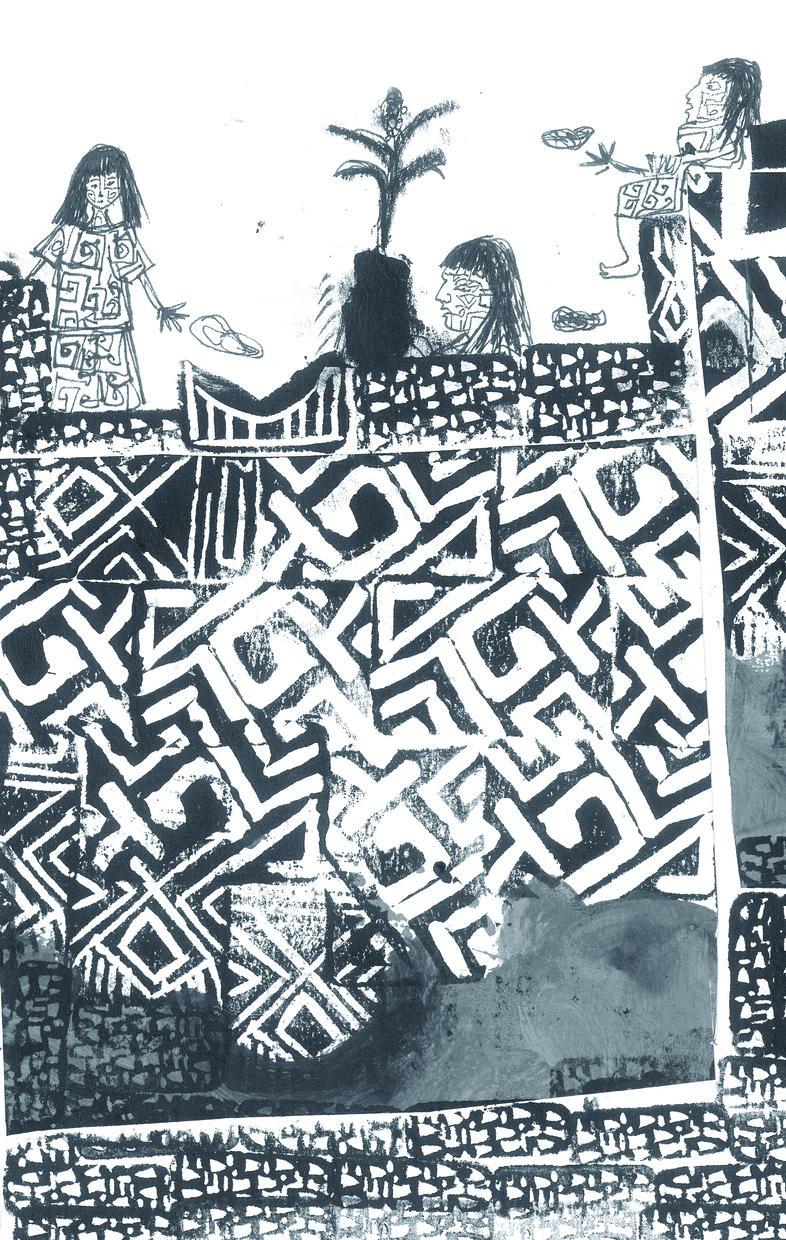
\includegraphics[width=138mm]{./imgs/img2.pdf}
\end{figure}

\chapter*{}

%\mbox{}\vspace*{\fill}
\vspace*{-\baselineskip}

% \begin{verse}
% Quando a velha vivia com\\
% a família, desperdiçava-se\\
% muito milho verde.\\
% Ela queria virar tatu, pois\\
% não podia comer o milho verde,\\
% visto que a família lhe dizia:\\
% --- Ô, velha, você só fica\\
% comendo o nosso milho verde.\\
% Ela respondia:\\
% --- Como só milho verde, por\\
% não poder comer milho seco.\\
% Não tenho dente.\\
% A mulher respondeu isso\\
% e ficou pensando no que\\
% a família lhe disse.
% \end{verse}

% \begin{verse}
% \textit{Hawen nabube hiwea,\\
% mawa xeki pati txakaaya.\\
% Yuxabudan yaix katsidan\\
% eskani kiaki. Haska waxun,\\
% pitima, xeki patxi besti piaya,\\
% hawen nabun itxaa:\\
% --- Yuxabun, min en xeki\\
% patxi besti piai, aka.\\
% Yuxabu yuikin:\\
% --- En haska waxun piti kuxi\\
% pitima. En xeta uma, en xeta\\
% umabin. Ainbun yuia, ainbu\\
% ninkaxun.}
% \end{verse}

\letra{Q}{uando} a velha vivia com
a família, desperdiçava-se
muito milho verde.
Ela queria virar tatu, pois
não podia comer o milho verde,
visto que a família lhe dizia:\break
--- Ô, velha, você só fica
comendo o nosso milho verde.
Ela respondia:\break
--- Como só milho verde, por
não poder comer milho seco.
Não tenho dente.\break
A mulher respondeu isso
e ficou pensando no que
a família lhe disse.

\vspace{2em}

\letra{H}{awen} nabube hiwea,
mawa xeki pati txakaaya.
Yuxabudan yaix katsidan
eskani kiaki. Haska waxun,
pitima, xeki patxi besti piaya,
hawen nabun itxaa:\break
--- Yuxabun, min en xeki
patxi besti piai, aka.
Yuxabu yuikin:\break
--- En haska waxun piti kuxi
pitima. En xeta uma, en xeta
umabin.\break
Ainbun yuia, ainbu
ninkaxun.

\vspace*{\fill}

\pagebreak
\thispagestyle{empty}
\begin{figure}
\vspace*{-.9cm}
\hspace*{-2.5cm}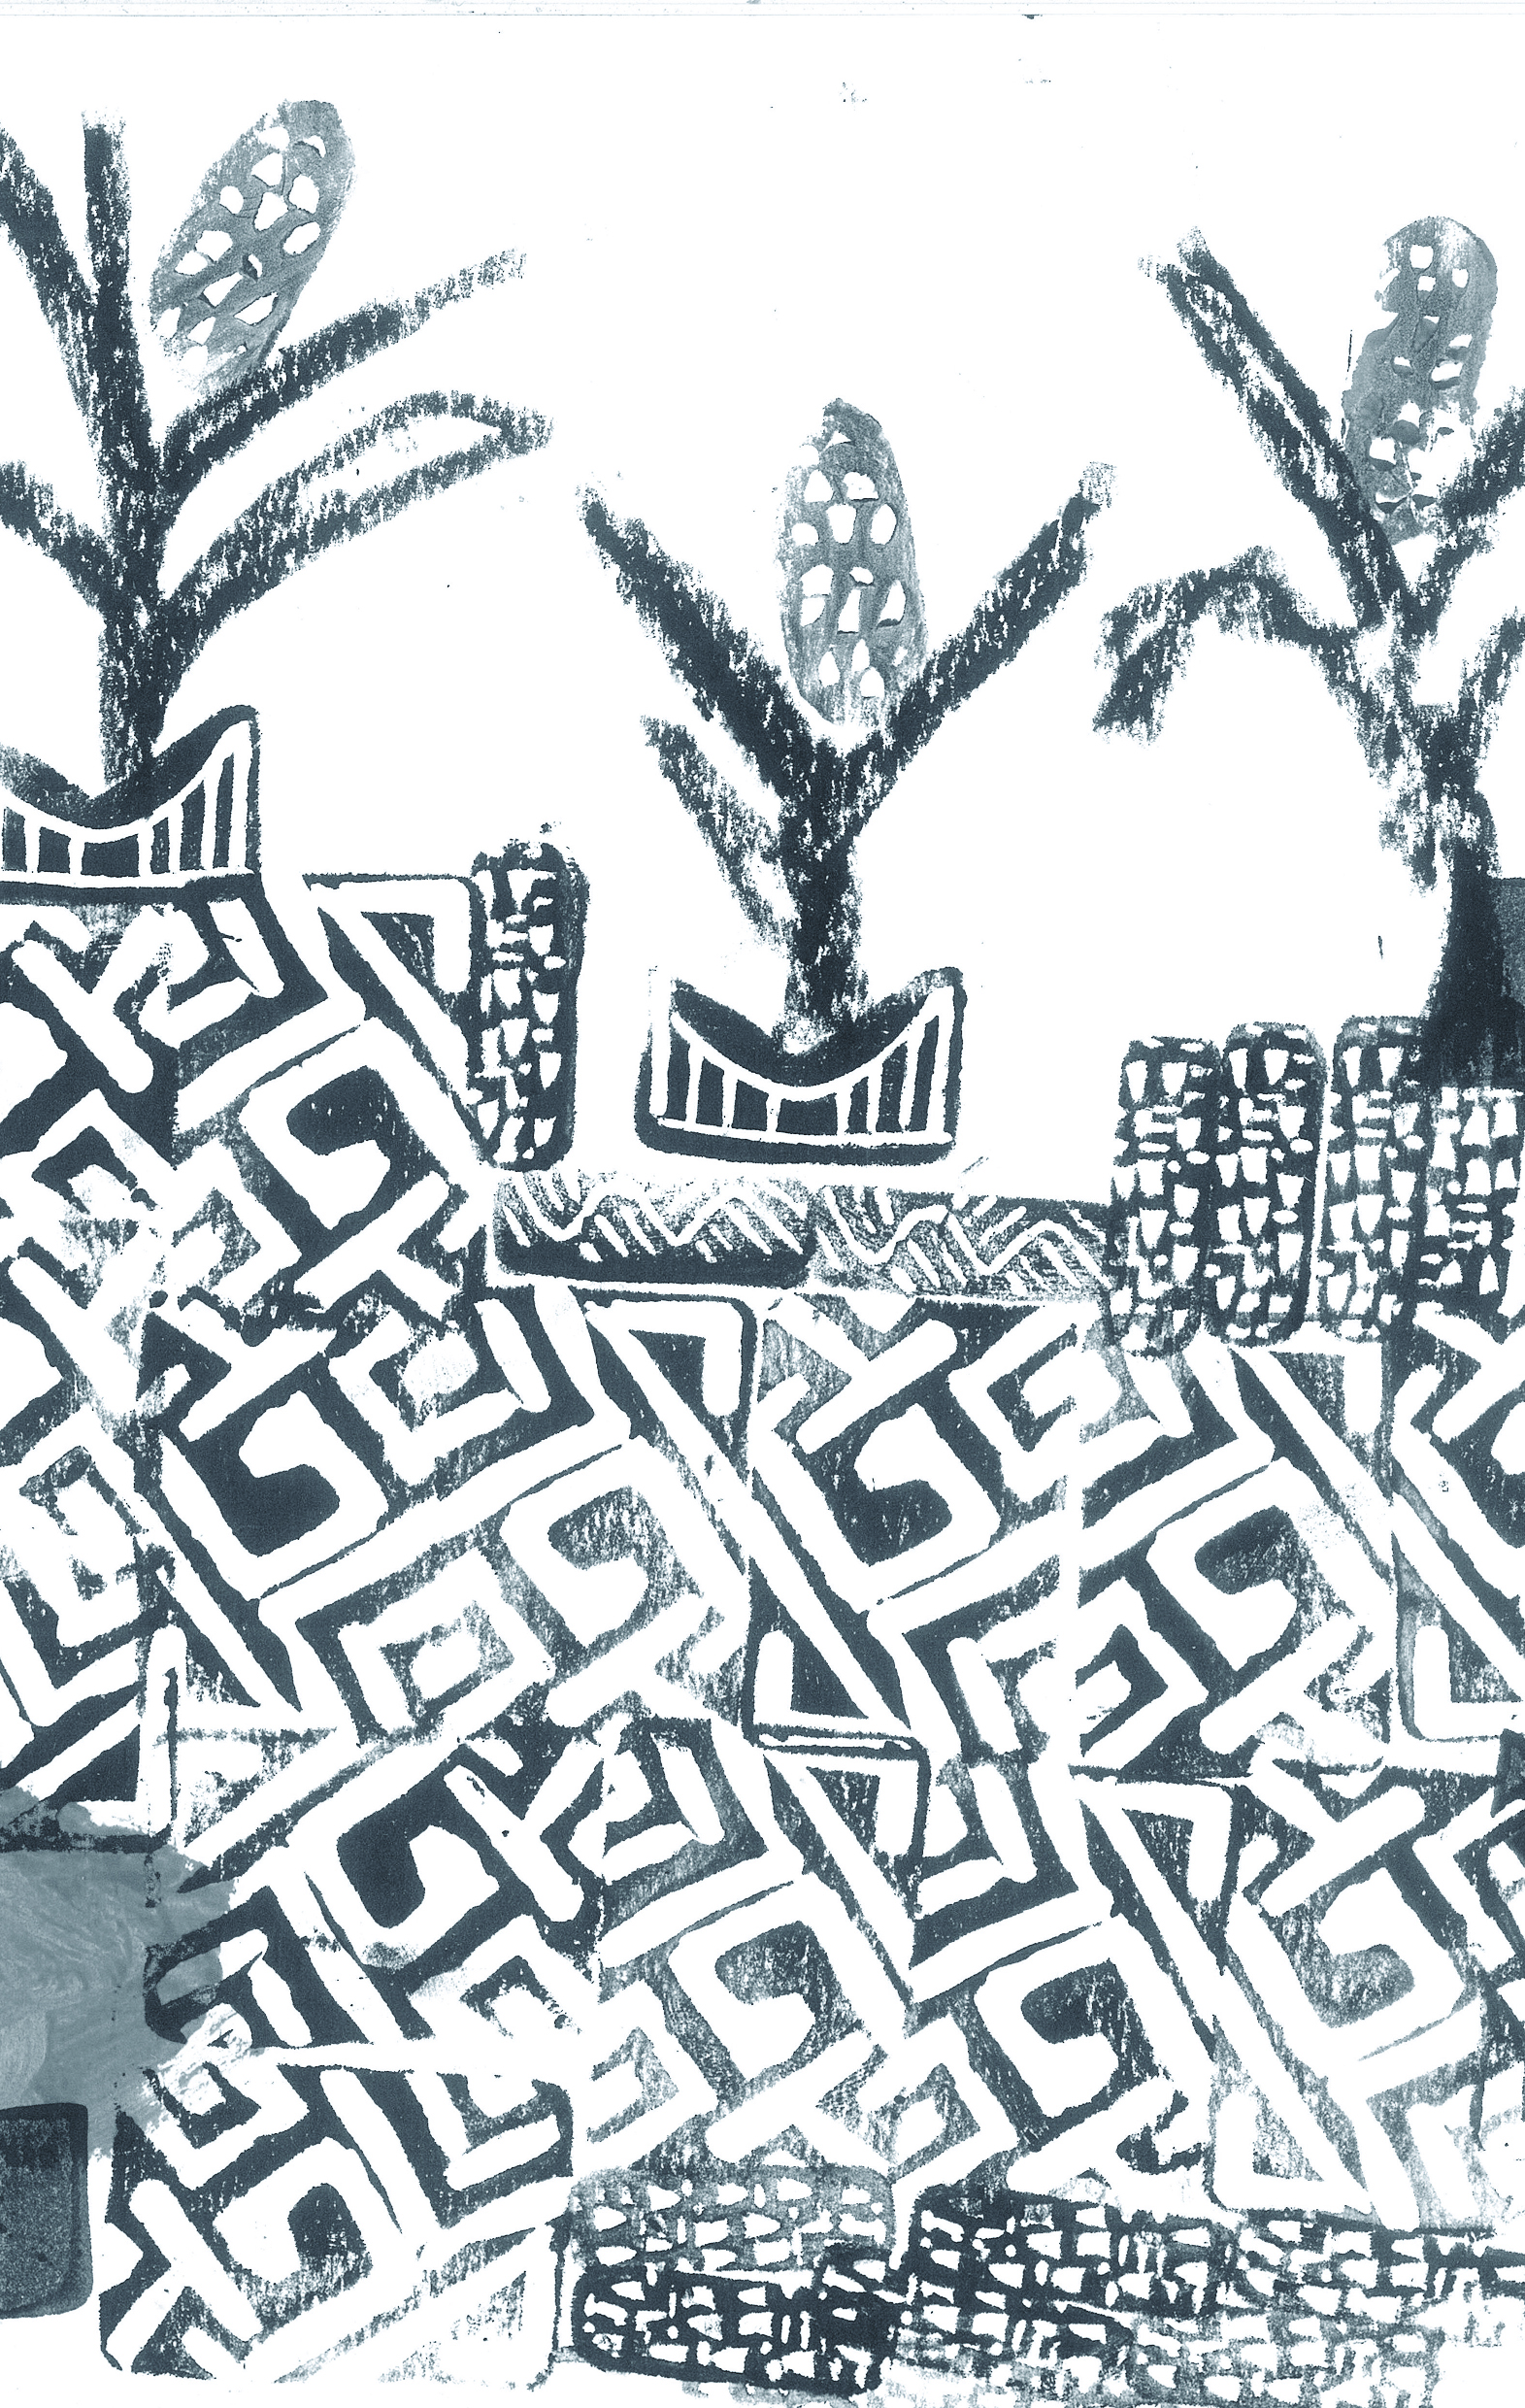
\includegraphics[width=143mm]{./imgs/img3.pdf}
\end{figure}

\chapter*{}

\vspace*{-\baselineskip}
%\mbox{}\vspace*{\fill}

% \begin{verse}
% Então ela foi sozinha mata\\
% adentro e, ao voltar, à\\
% tardezinha, disse à sua filha:\\
% --- Filha, eu vou virar tatu. Sou\\
% desdentada e por isso não posso\\
% comer milho verde. Vou embora.\\
% A filha respondeu-lhe:\\
% --- Mamãe, é por isso que\\
% você não pode comer?\\
% --- Minha filha, é. É por isso que\\
% não posso comer — respondeu-lhe.\\
% A filha replicou:\\
% --- Mamãe, então coma\\
% só milho verde!
% \end{verse}

% \begin{verse}
% \textit{Hanunkain, yuxabu ni medan\\
% ha mesti kaa, badi kaaya\\
% huxun, hawen bake yuia:\\
% --- En bake, eadan en yaixi kaai. En\\
% xeta uma. Haska waxun,\\
% piti kuxi pitima, en ikai, aka.\\
% Hawen bake yuikin:\\
% --- En ewan, min haska waxun\\
% pitimamen, aka. En bake, en haska\\
% waxun, pitimabin, aka.\\
% Hawen bake yuia:\\
% --- Ewan, xeki patxi\\
% besti piwe, aka.}
% \end{verse}

\letra{E}{ntão} ela foi sozinha mata
adentro e, ao voltar, à
tardezinha, disse à sua filha:\break
--- Filha, eu vou virar tatu. Sou
desdentada e por isso não posso
comer milho verde. Vou embora.
A filha respondeu-lhe:\break
--- Mamãe, é por isso que
você não pode comer?\break
--- Minha filha, é. É por isso que
não posso comer, respondeu-lhe.
A filha replicou:\break
--- Mamãe, então coma
só milho verde!

\vspace{2em}

\letra{H}{anunkain}, yuxabu ni medan
ha mesti kaa, badi kaaya
huxun, hawen bake yuia:\break
--- En bake, eadan en yaixi kaai. En
xeta uma. Haska waxun,
piti kuxi pitima, en ikai, aka.
Hawen bake yuikin:\break
--- En ewan, min haska waxun
pitimamen, aka. En bake, en haska
waxun, pitimabin, aka.
Hawen bake yuia:\break
--- Ewan, xeki patxi
besti piwe, aka.

\vspace*{\fill}

\pagebreak
\thispagestyle{empty}
\begin{figure}
\vspace*{-.5cm}
\hspace*{-2.2cm}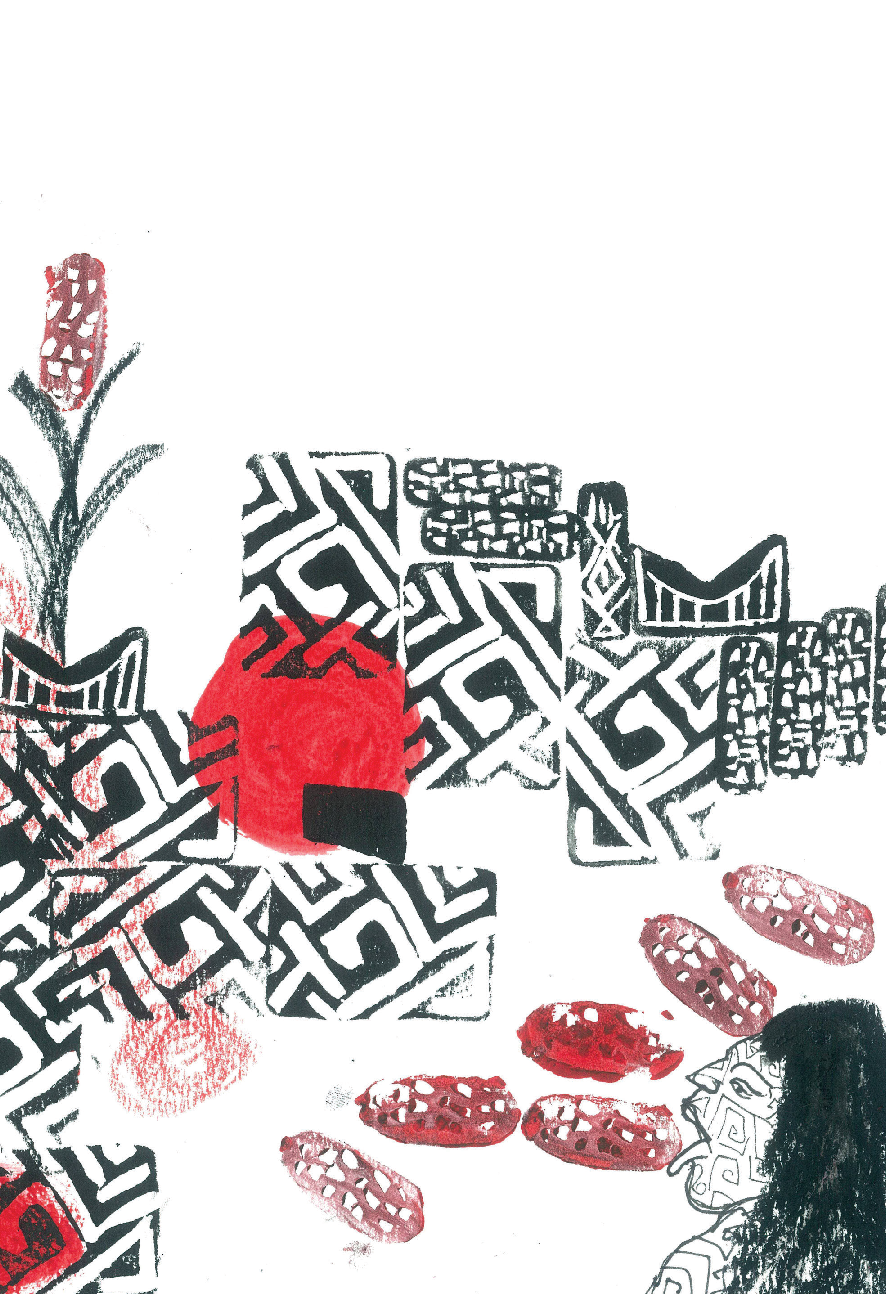
\includegraphics[width=138mm]{./imgs/img4.pdf}
\end{figure}

\chapter*{}

\mbox{}\vspace*{\fill}

% \begin{verse}
% A velha só comia milho\\
% verde por não poder comer\\
% milho seco, que é duro.\\
% Quando acabou o milho verde\\
% do roçado deles, os homens\\
% estavam zangados\\
% e lhe disseram:\\
% --- Velha, você acabou com o\\
% nosso roçado de milho verde.\\
% \end{verse}

% \begin{verse}
% \textit{Yuxabun xeki patxi besti piaya.\\
% Haska waxun, piti kuxi pitima.\\
% Hatun bai xeki patxi keyun waaya,\\
% hunibun sinaxun, yuxabu yuikin:\\
% --- Yuxabun, min en xeki\\
% patxi bai keyuna, aka.\\}
% \end{verse}

\letra{A}{velha} só comia milho
verde por não poder comer
milho seco, que é duro.
Quando acabou o milho verde
do roçado deles, os homens
estavam zangados
e lhe disseram:\break
--- Velha, você acabou com o
nosso roçado de milho verde.

\vspace{2em}

\letra{Y}{uxabun} xeki patxi besti piaya.
Haska waxun, piti kuxi pitima.
Hatun bai xeki patxi keyun waaya,
hunibun sinaxun, yuxabu yuikin:\break
--- Yuxabun, min en xeki
patxi bai keyuna, aka.

\vspace*{\fill}

\pagebreak
\thispagestyle{empty}
\begin{figure}
\vspace*{-1.3cm}
\hspace*{-2.5cm}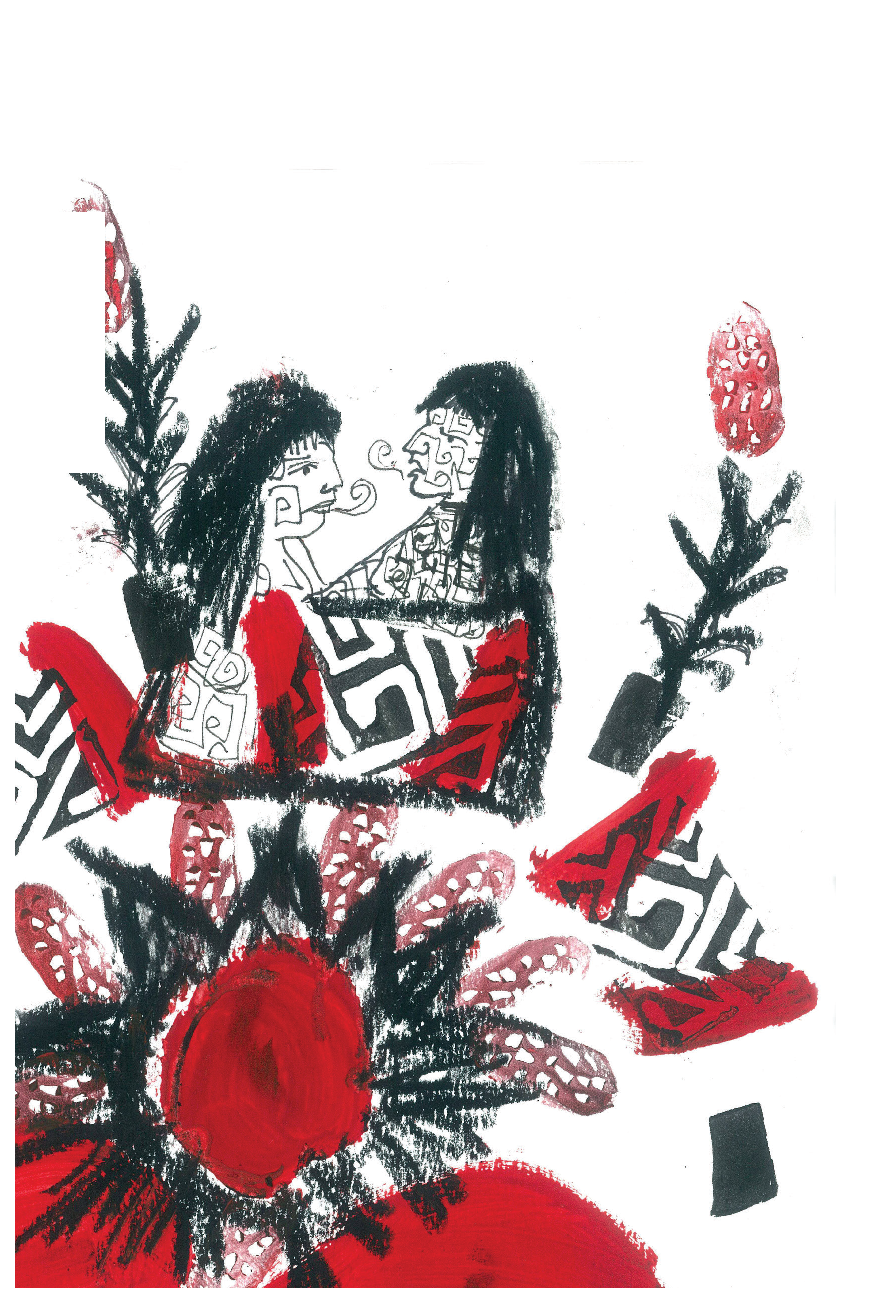
\includegraphics[width=145mm]{./imgs/img5.pdf}
\end{figure}

\chapter*{}

% \begin{verse}
% Ela lhes respondeu:\\
% --- É por não poder comer milho\\
% seco. Sou desdentada. Por\\
% sinal, minha filha me disse:\\
% \textit{Mamãe, coma milho verde!}, e\\
% respondi \textit{Vou comer, sim}.\\
% Assim disse a velha. Mas os\\
% homens retrucaram-lhe:\\
% --- Pare de comer o nosso milho!
% \end{verse}

% \begin{verse}
% \textit{Yuxabu yuikin:\\
% --- En haska waxun, piti kuxi\\
% pitima, en ikai, aka. Eadan,\\
% en xeta umabin, aka.\\
% Habia en baken:\\
% --- Xeki patxi piwe, ewan,\\
% yui. En piai, aka.\\
% Yuxabun haska waa.\\
% Hunibun yuxabu yuikin:\\
% --- En xeki ea keyunyamawe, aka.}
% \end{verse}

\letra{E}{la} lhes respondeu:\break
--- É por não poder comer milho
seco. Sou desdentada. Por
sinal, minha filha me disse:\break
--- Mamãe, coma milho verde!\break
E respondi:\break
--- Vou comer, sim.
Assim disse a velha. Mas os
homens retrucaram-lhe:\break
--- Pare de comer o nosso milho!

\vspace{2em}

\letra{Y}{uxabu} yuikin:\break
--- En haska waxun, piti kuxi
pitima, en ikai, aka. Eadan,
en xeta umabin, aka.
Habia en baken:\break
--- Xeki patxi piwe, ewan,
yui.\break
En piai, aka. Yuxabun haska waa.
Hunibun yuxabu yuikin:\break
--- En xeki ea keyunyamawe, aka.

\vspace*{\fill}

\pagebreak
\thispagestyle{empty}
\begin{figure}
\vspace*{-2.5cm}
\hspace*{-2.8cm}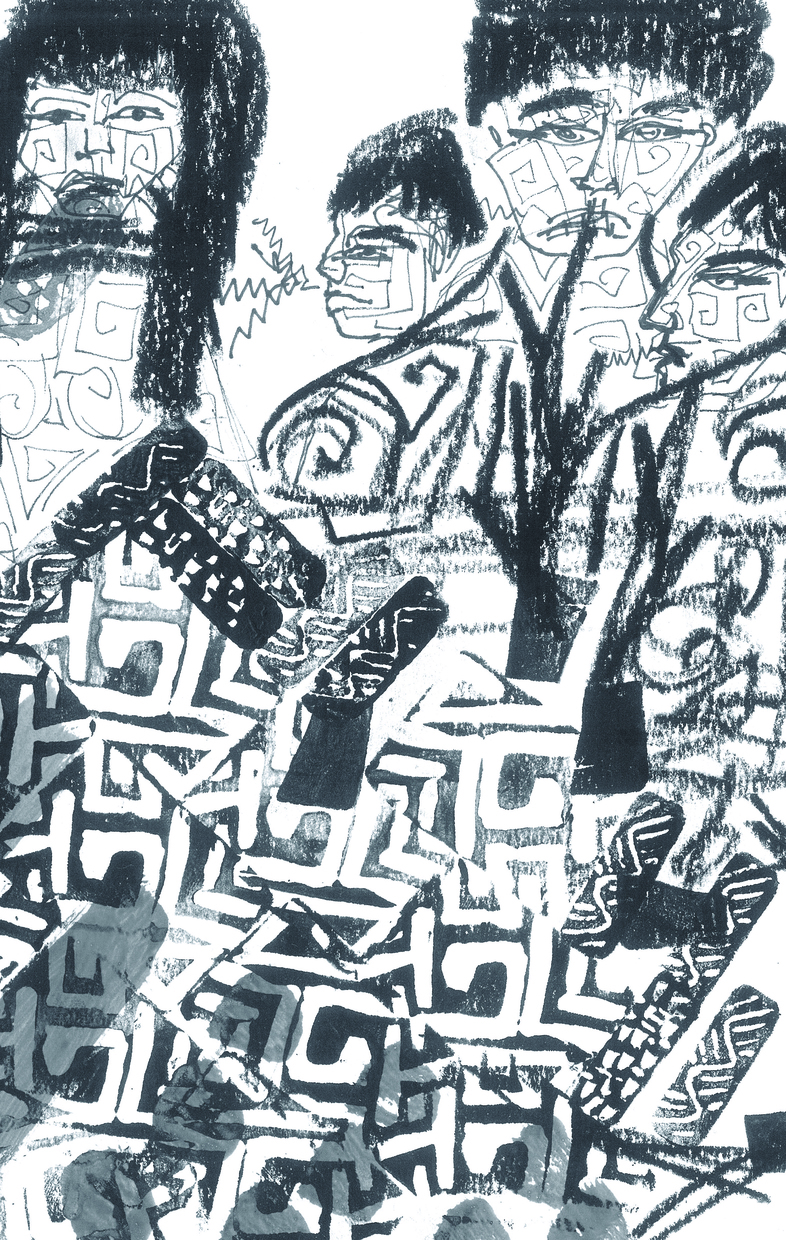
\includegraphics[width=152mm]{./imgs/img6.pdf}
\end{figure}

\chapter*{}

\mbox{}\vspace*{\fill}

% \begin{verse}
% Não podendo mais comer milho verde,\\
% a velha chorou e quis virar tatu.\\
% Foi sozinha para o mato e cavou um buraco.
% \end{verse}

% \begin{verse}
% \textit{Yuxabu haska waa, ana hawa pitima,\\
% kaxaaya. Yuxabu yaixi ka katsi eskani kiaki.\\
% Ha mesti ni medan kaxun, kini waaya.}
% \end{verse}

\letra{N}{ão} podendo mais comer milho verde,
a velha chorou e quis virar tatu.
Foi sozinha para o mato e cavou um buraco.

\vspace{2em}

\letra{Y}{uxabu} haska waa, ana hawa pitima,
kaxaaya. Yuxabu yaixi ka katsi eskani kiaki.
Ha mesti ni medan kaxun, kini waaya.

\vspace*{\fill}

\pagebreak
\thispagestyle{empty}
\begin{figure}
\vspace*{-.5cm}
\hspace*{-2.2cm}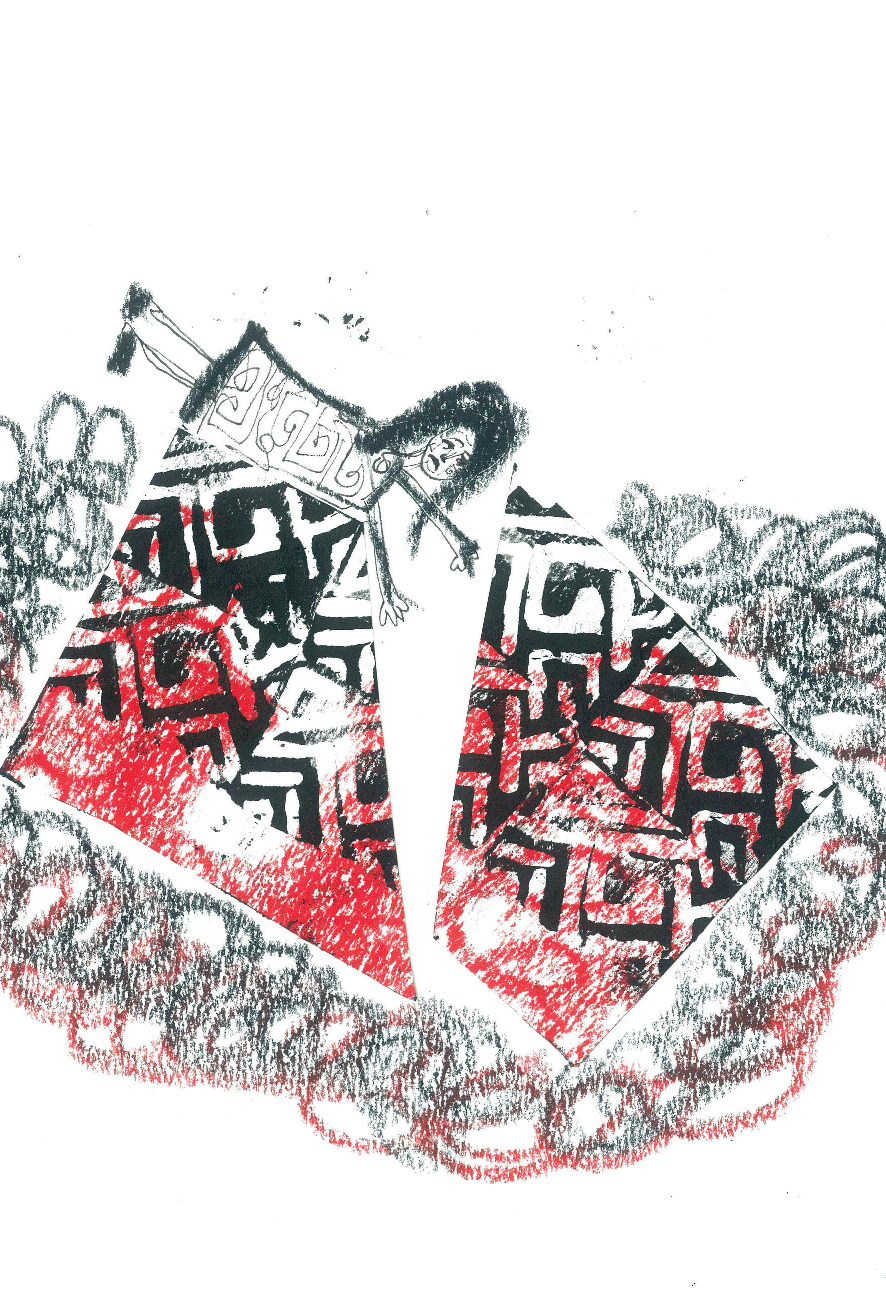
\includegraphics[width=138mm]{./imgs/img7.pdf}
\end{figure}

\chapter*{}

\mbox{}\vspace*{\fill}

% \begin{verse}
% Um homem que havia ido caçar a viu\\
% cavando o buraco, aproximou-se\\
% dela e lhe perguntou:\\
% --- Ei, velha, por que você\\
% está cavando um buraco?\\
% --- É porque não posso comer milho seco.\\
% Só posso comer milho verde. Mas como\\
% esculhambaram comigo, vim cavar um\\
% buraco para ser tatu, respondeu.\\
% O homem a escutou e ficou pensativo,\\
% chorando tristemente.
% \end{verse}

% \begin{verse}
% \textit{Huni piaya kaxun, yuxabun kini\\
% waa, betxia, hunin yuxabu yukaa:\\
% --- Yuxabun, min hawa\\
% katsi kini waai? aka.\\
% --- En haska waxun, piti kuxi\\
% pitima, xeki patxi besti en piaya,\\
% ea itxabu, huxun, en kini waai\\
% yaix katsidan, aka.\\
% Hunin ninkaa, hawen\\
% dabanen iki, kaxaaya.}
% \end{verse}

\letra{U}{m} homem que havia ido caçar a viu
cavando o buraco, aproximou-se
dela e lhe perguntou:\break
--- Ei, velha, por que você
está cavando um buraco?\break
--- É porque não posso comer milho seco.
Só posso comer milho verde. Mas como
esculhambaram comigo, vim cavar um
buraco para ser tatu, respondeu.\break
O homem a escutou e ficou pensativo,
chorando tristemente.

\vspace{2em}

\letra{H}{uni} piaya kaxun, yuxabun kini
waa, betxia, hunin yuxabu yukaa:\break
--- Yuxabun, min hawa
katsi kini waai? aka.\break
--- En haska waxun, piti kuxi
pitima, xeki patxi besti en piaya,
ea itxabu, huxun, en kini waai
yaix katsidan, aka.\break
Hunin ninkaa, hawen
dabanen iki, kaxaaya.

\vspace*{\fill}

\pagebreak
\thispagestyle{empty}
\begin{figure}
\vspace*{-2cm}
\hspace*{-2.8cm}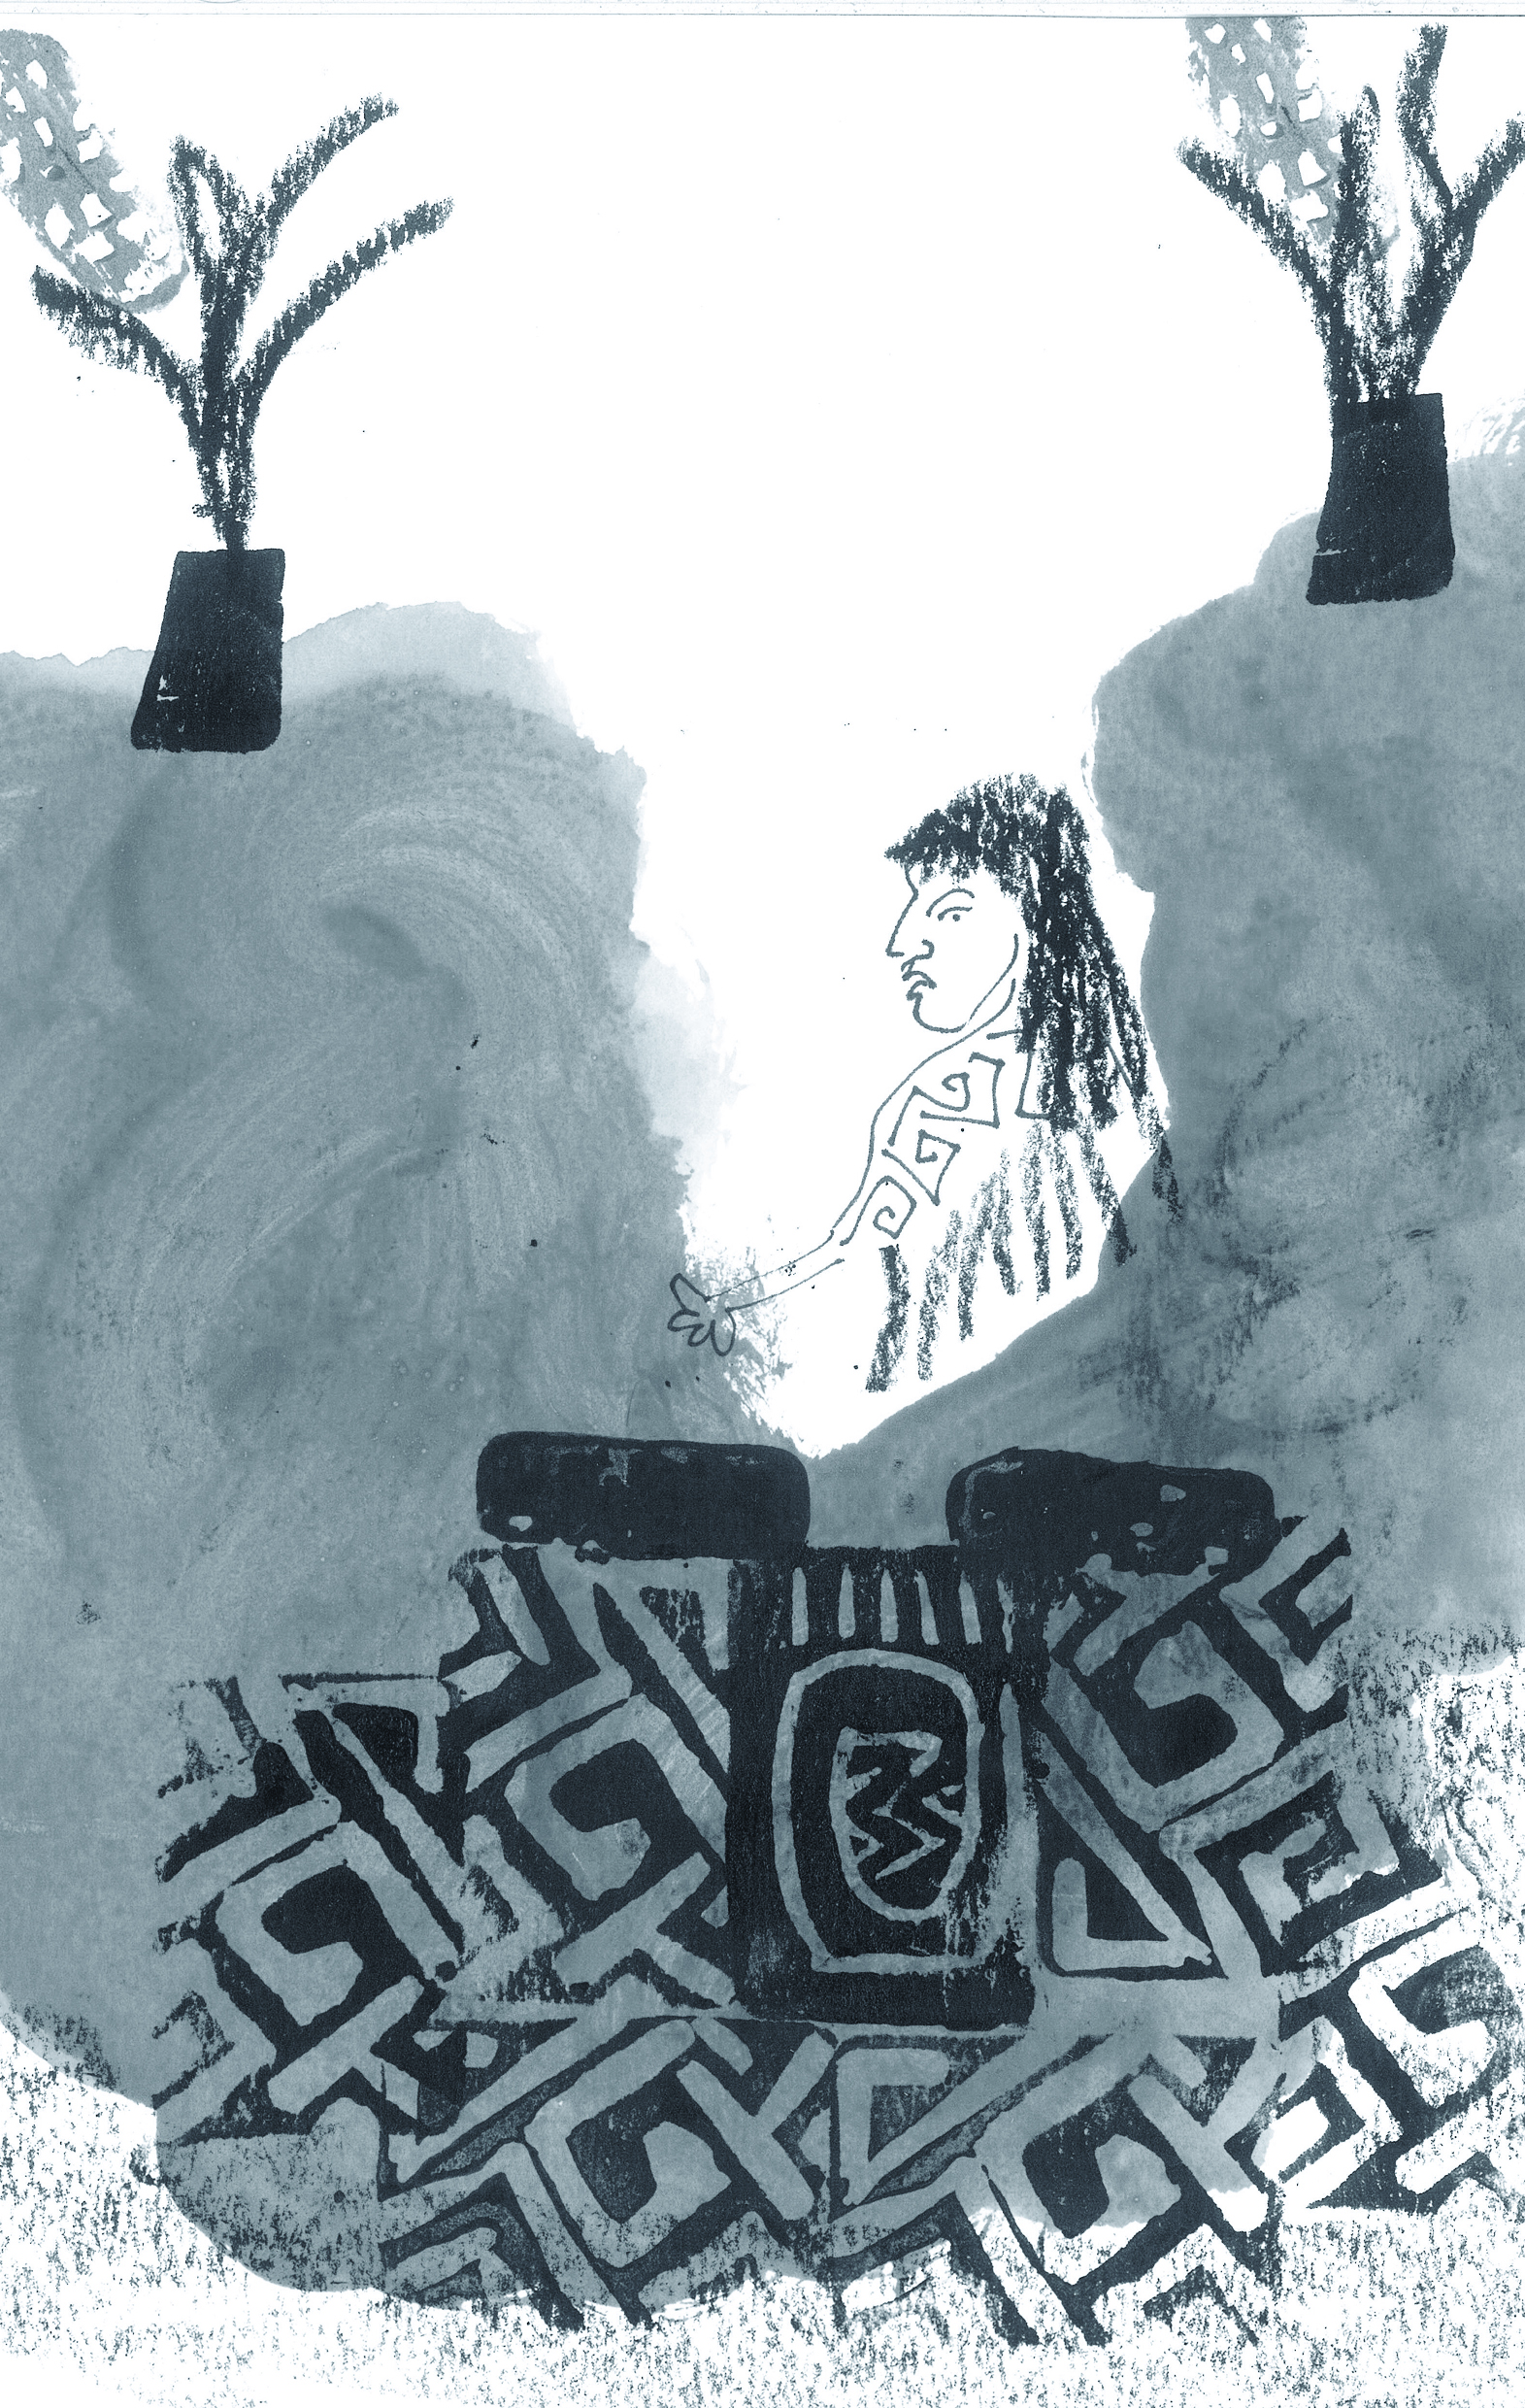
\includegraphics[width=150mm]{./imgs/img8.pdf}
\end{figure}

\chapter*{}

\mbox{}\vspace*{\fill}

% \begin{verse}
% Ao regressar, pergunto\\
% à família dela:\\
% --- Por que vocês\\
% esculhambaram com a velha?\\
% --- Esculhambei porque ela só\\
% comia o milho verde do meu\\
% roçado. Eu a insultei e\\
% ela foi embora.\\
% --- A velha foi para lá cavar\\
% buraco, eu a vi. Ela quer virar\\
% tatu — disse o caçador.
% \end{verse}

% \begin{verse}
% \textit{Haska wabidani, hukidan,\\
% hawen nabu yuia:\\
% --- En nabun, mi hawa\\
% katsi yuxabu\\
% itxa kamen, aka.\\
% --- Habia en xeki patxi\\
% ea pianaya,\\
% en itxaa, kaaki, aka.\\
% --- Yuxabudan uani kini\\
% waai, en uinbidanxuki,\\
% yaix katsidan, aka.}
% \end{verse}

\letra{A}{o} regressar, pergunto
à família dela:\break
--- Por que vocês
esculhambaram com a velha?\break
--- Esculhambei porque ela só
comia o milho verde do meu
roçado. Eu a insultei e
ela foi embora.\break
--- A velha foi para lá cavar
buraco, eu a vi. Ela quer virar
tatu — disse o caçador.

\vspace{2em}

\letra{H}{aska} wabidani, hukidan,
hawen nabu yuia:\break
--- En nabun, mi hawa
katsi yuxabu
itxa kamen, aka.\break
--- Habia en xeki patxi
ea pianaya,
en itxaa, kaaki, aka.\break
--- Yuxabudan uani kini
waai, en uinbidanxuki,
yaix katsidan, aka.

\vspace*{\fill}

\pagebreak
\thispagestyle{empty}
\begin{figure}
\vspace*{-.5cm}
\hspace*{-2.2cm}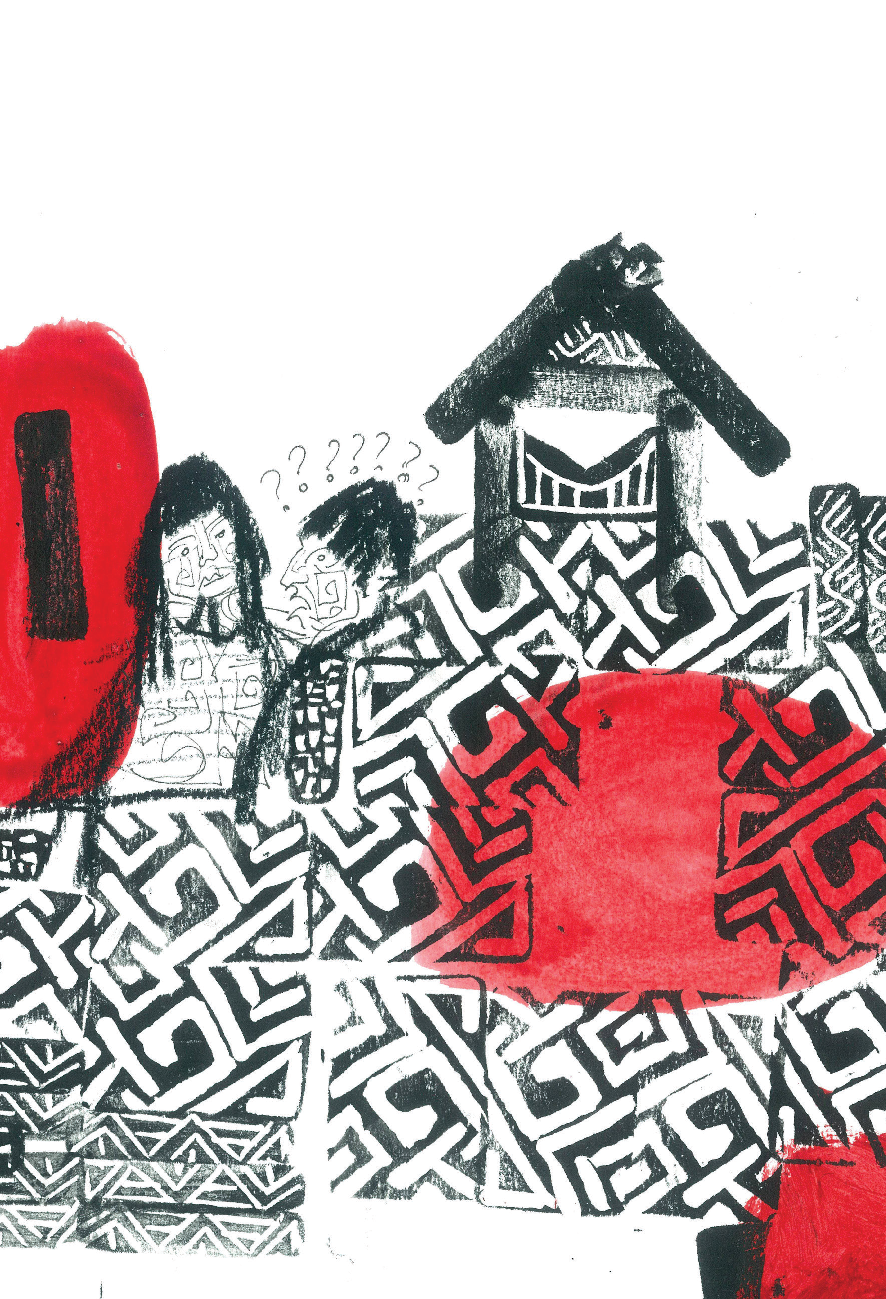
\includegraphics[width=138mm]{./imgs/img9.pdf}
\end{figure}

\chapter*{}

\mbox{}\vspace*{\fill}

% \begin{verse}
% O caçador disse ao seu\\
% filho que estava chorando:\\
% --- A velha que vocês esculhambaram\\
% já virou tatu. Ela já tem rabo, casco\\
% nas costas, casco na cabeça. Virou\\
% todinha tatu. A velha sente falta\\
% do filho. \textit{Vou buscá-lo}, disse a\\
% si mesma. Chamou por ele, gritando\\
% \textit{ruu}, fazendo barulho de tatu.
% \end{verse}

% \begin{verse}
% \textit{Hawen bake yuia, kaxaaya.\\
% --- Yuxabu ma yaixa. Hanunkain, hinayatan,\\
% pexakayatan, nuxakayatan, buxakayatan.\\
% Haska wakin, keyua. Yuxabu hawen bake\\
% manui: \emph{En bake itannun} ika. \emph{Huu} aka.}
% \end{verse}

\letra{O}{caçador} disse ao seu
filho que estava chorando:\break
--- A velha que vocês esculhambaram
já virou tatu. Ela já tem rabo, casco
nas costas, casco na cabeça. Virou
todinha tatu. A velha sente falta
do filho.\break 
\textit{Vou buscá-lo}, disse a
si mesma. Chamou por ele, gritando
\textit{ruu}, fazendo barulho de tatu.

\vspace{2em}

\letra{H}{awen} bake yuia, kaxaaya.\break
--- Yuxabu ma yaixa. Hanunkain, hinayatan,
pexakayatan, nuxakayatan, buxakayatan.\break
Haska wakin, keyua. Yuxabu hawen bake
manui:\break 
\emph{En bake itannun} ika. \emph{Huu} aka.

\vspace*{\fill}

\pagebreak
\thispagestyle{empty}
\begin{figure}
\vspace*{-1cm}
\hspace*{-2.2cm}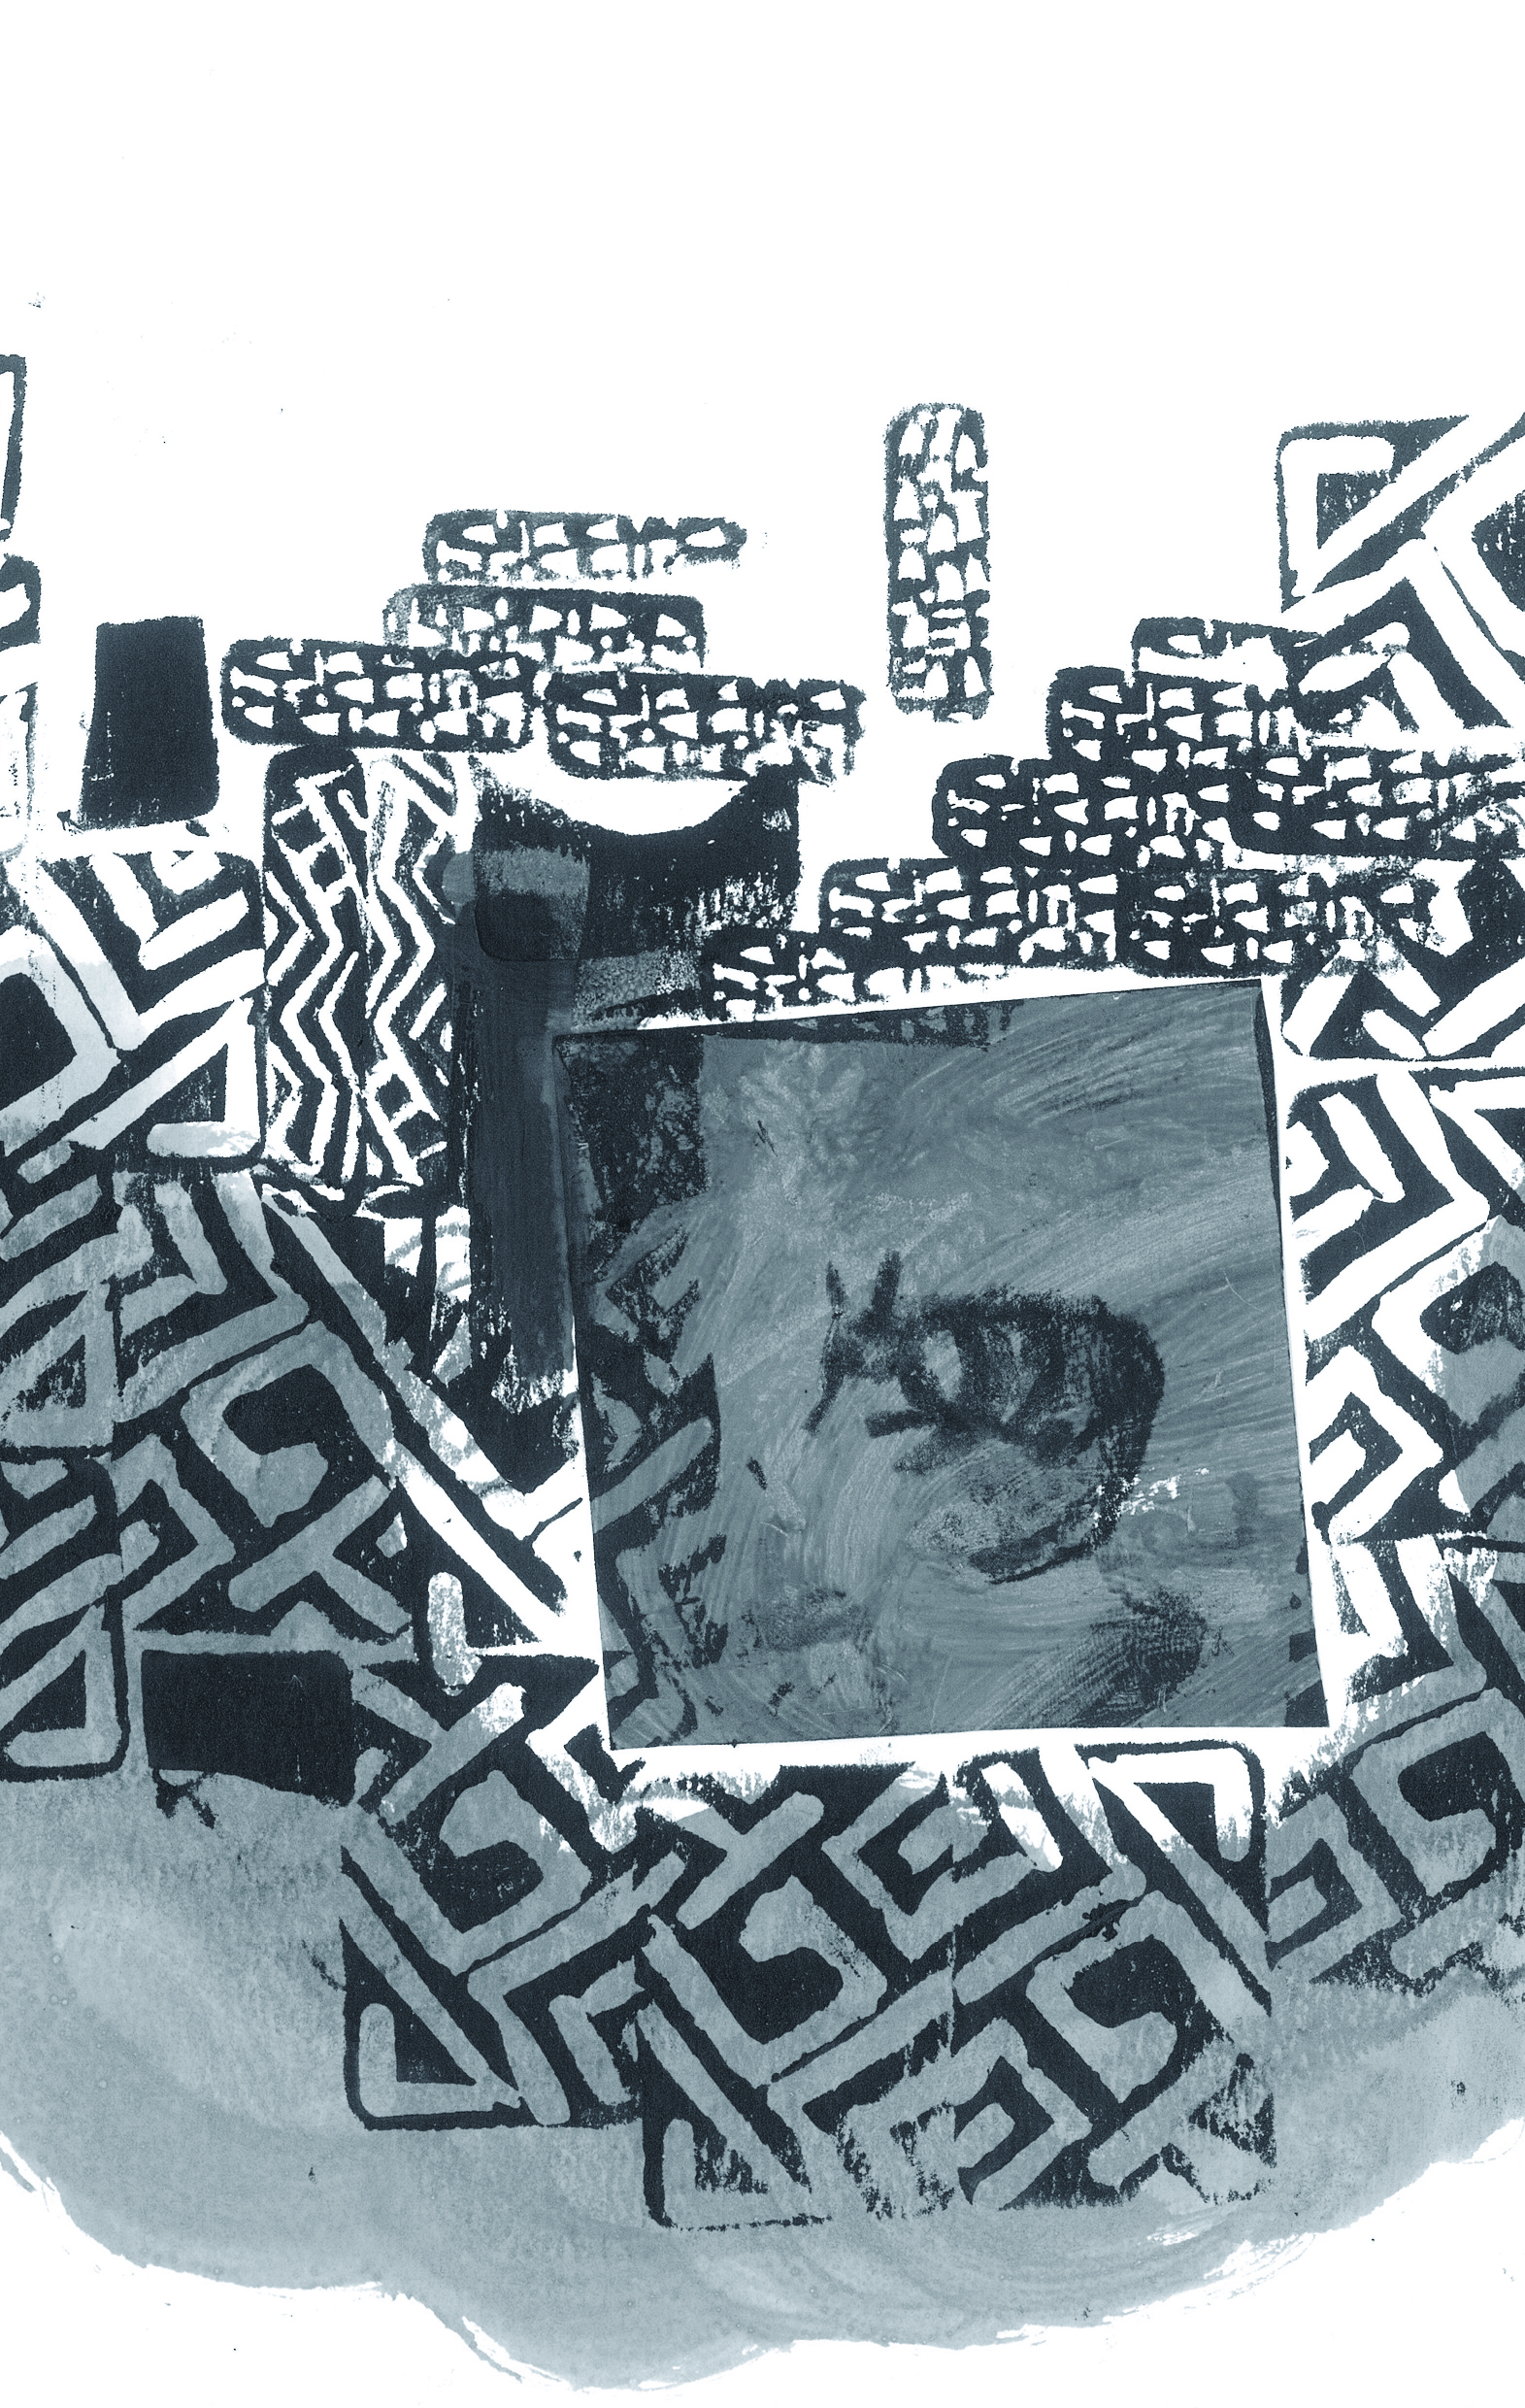
\includegraphics[width=138mm]{./imgs/img10.pdf}
\end{figure}

\chapter*{}

\mbox{}\vspace*{\fill}

% \begin{verse}
% O seu filho pequeno sentia falta\\
% da mãe, e chorava sem parar.\\
% Ele andava sozinho, chorando,\\
% de um lado para o outro.\\
% A velha ouviu o choro e pensou:\\
% --- O meu filho está chorando, vou vê-lo.\\
% Voltou à aldeia para vê-lo; lá estava ele\\
% sentado, chorando. Quando viu o tatu,\\
% alegrou-se, e o tatu lhe disse:\\
% --- Meu filho, eu vou te levar.
% \end{verse}

% \begin{verse}
% \textit{Hawen bake hawen ibu\\
% manui, kaxawankainkainaya.\\
% Hawen bake, ha mesti bai\\
% tanai, kaxakukuaya.\\
% Yuxabu kaxai ninkaa:\\
% --- En bake kaxaai, uintannun, ika.\\
% Huaya, bake pixta kaxai, tsauken,\\
% bake pixta yaix betxia, benimaaya.\\
% Yaixin bake pixta yuikin:\\
% --- En bake, en mia yuai, aka.}
% \end{verse}

\letra{O}{seu} filho pequeno sentia falta
da mãe, e chorava sem parar.
Ele andava sozinho, chorando,
de um lado para o outro.
A velha ouviu o choro e pensou:\break
--- O meu filho está chorando, vou vê-lo.
Voltou à aldeia para vê-lo; lá estava ele
sentado, chorando. Quando viu o tatu,
alegrou-se, e o tatu lhe disse:\break
--- Meu filho, eu vou te levar.

\vspace{2em}

\letra{H}{awen} bake hawen ibu
manui, kaxawankainkainaya.
Hawen bake, ha mesti bai
tanai, kaxakukuaya.
Yuxabu kaxai ninkaa:\break
--- En bake kaxaai, uintannun, ika.
Huaya, bake pixta kaxai, tsauken,
bake pixta yaix betxia, benimaaya.
Yaixin bake pixta yuikin:\break
--- En bake, en mia yuai, aka.

\vspace*{\fill}

\pagebreak
\thispagestyle{empty}
\begin{figure}
\vspace*{-.5cm}
\hspace*{-2.2cm}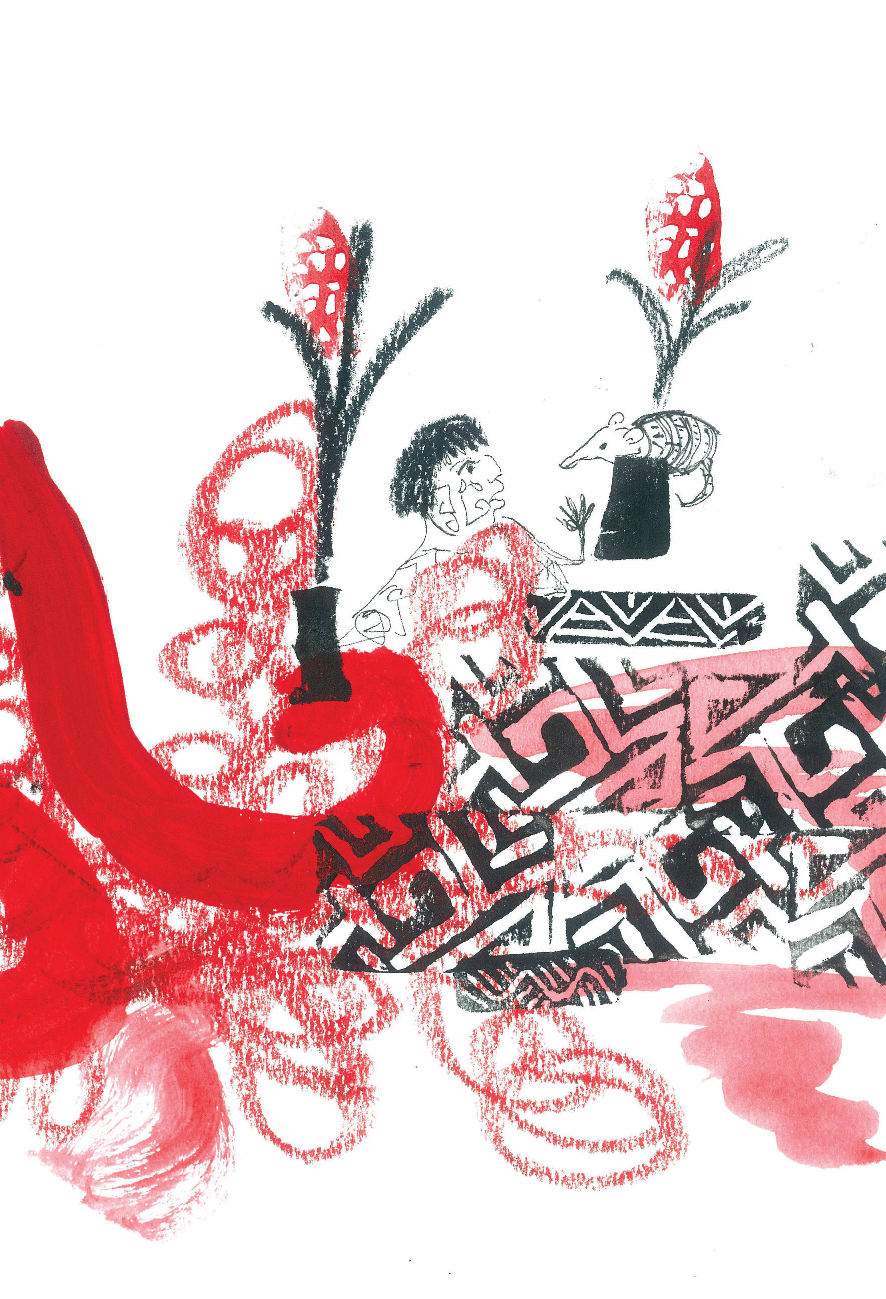
\includegraphics[width=138mm]{./imgs/img11.pdf}
\end{figure}

\chapter*{}

\mbox{}\vspace*{\fill}

% \begin{verse}
% A criança que estava\\
% sentada ficou contente.\\
% Então a velha levou o menino\\
% para morar dentro do buraco.\\
% Ela lhe fez o rabo, o casco das\\
% costas, o casco da cabeça.\\
% E a criança ficou feliz.\\
% A velha havia feito a mesma\\
% coisa para virar tatu.
% \end{verse}

% \begin{verse}
% \textit{Bake pixta benimaai, tsauken.\\
% Hanunkain, yuxabun bake pixta\\
% hawen hiwe medan yukin.\\
% Bake pixta hina waxun, pexaka\\
% waxun, buxaka waxun.\\
% Haska waxun, bake pixta\\
% benimani kiaki.\\
% Yuxabudan eskani kiaki,\\
% yaix katsidan.}
% \end{verse}

\letra{A}{criança} que estava
sentada ficou contente.
Então a velha levou o menino
para morar dentro do buraco.
Ela lhe fez o rabo, o casco das
costas, o casco da cabeça.
E a criança ficou feliz.
A velha havia feito a mesma
coisa para virar tatu.

\vspace{2em}

\letra{B}{ake} pixta benimaai, tsauken.
Hanunkain, yuxabun bake pixta
hawen hiwe medan yukin.
Bake pixta hina waxun, pexaka
waxun, buxaka waxun.
Haska waxun, bake pixta
benimani kiaki.
Yuxabudan eskani kiaki,
yaix katsidan.

\vspace*{\fill}

\pagebreak
\thispagestyle{empty}
\begin{figure}
\vspace*{-2cm}
\hspace*{-2.8cm}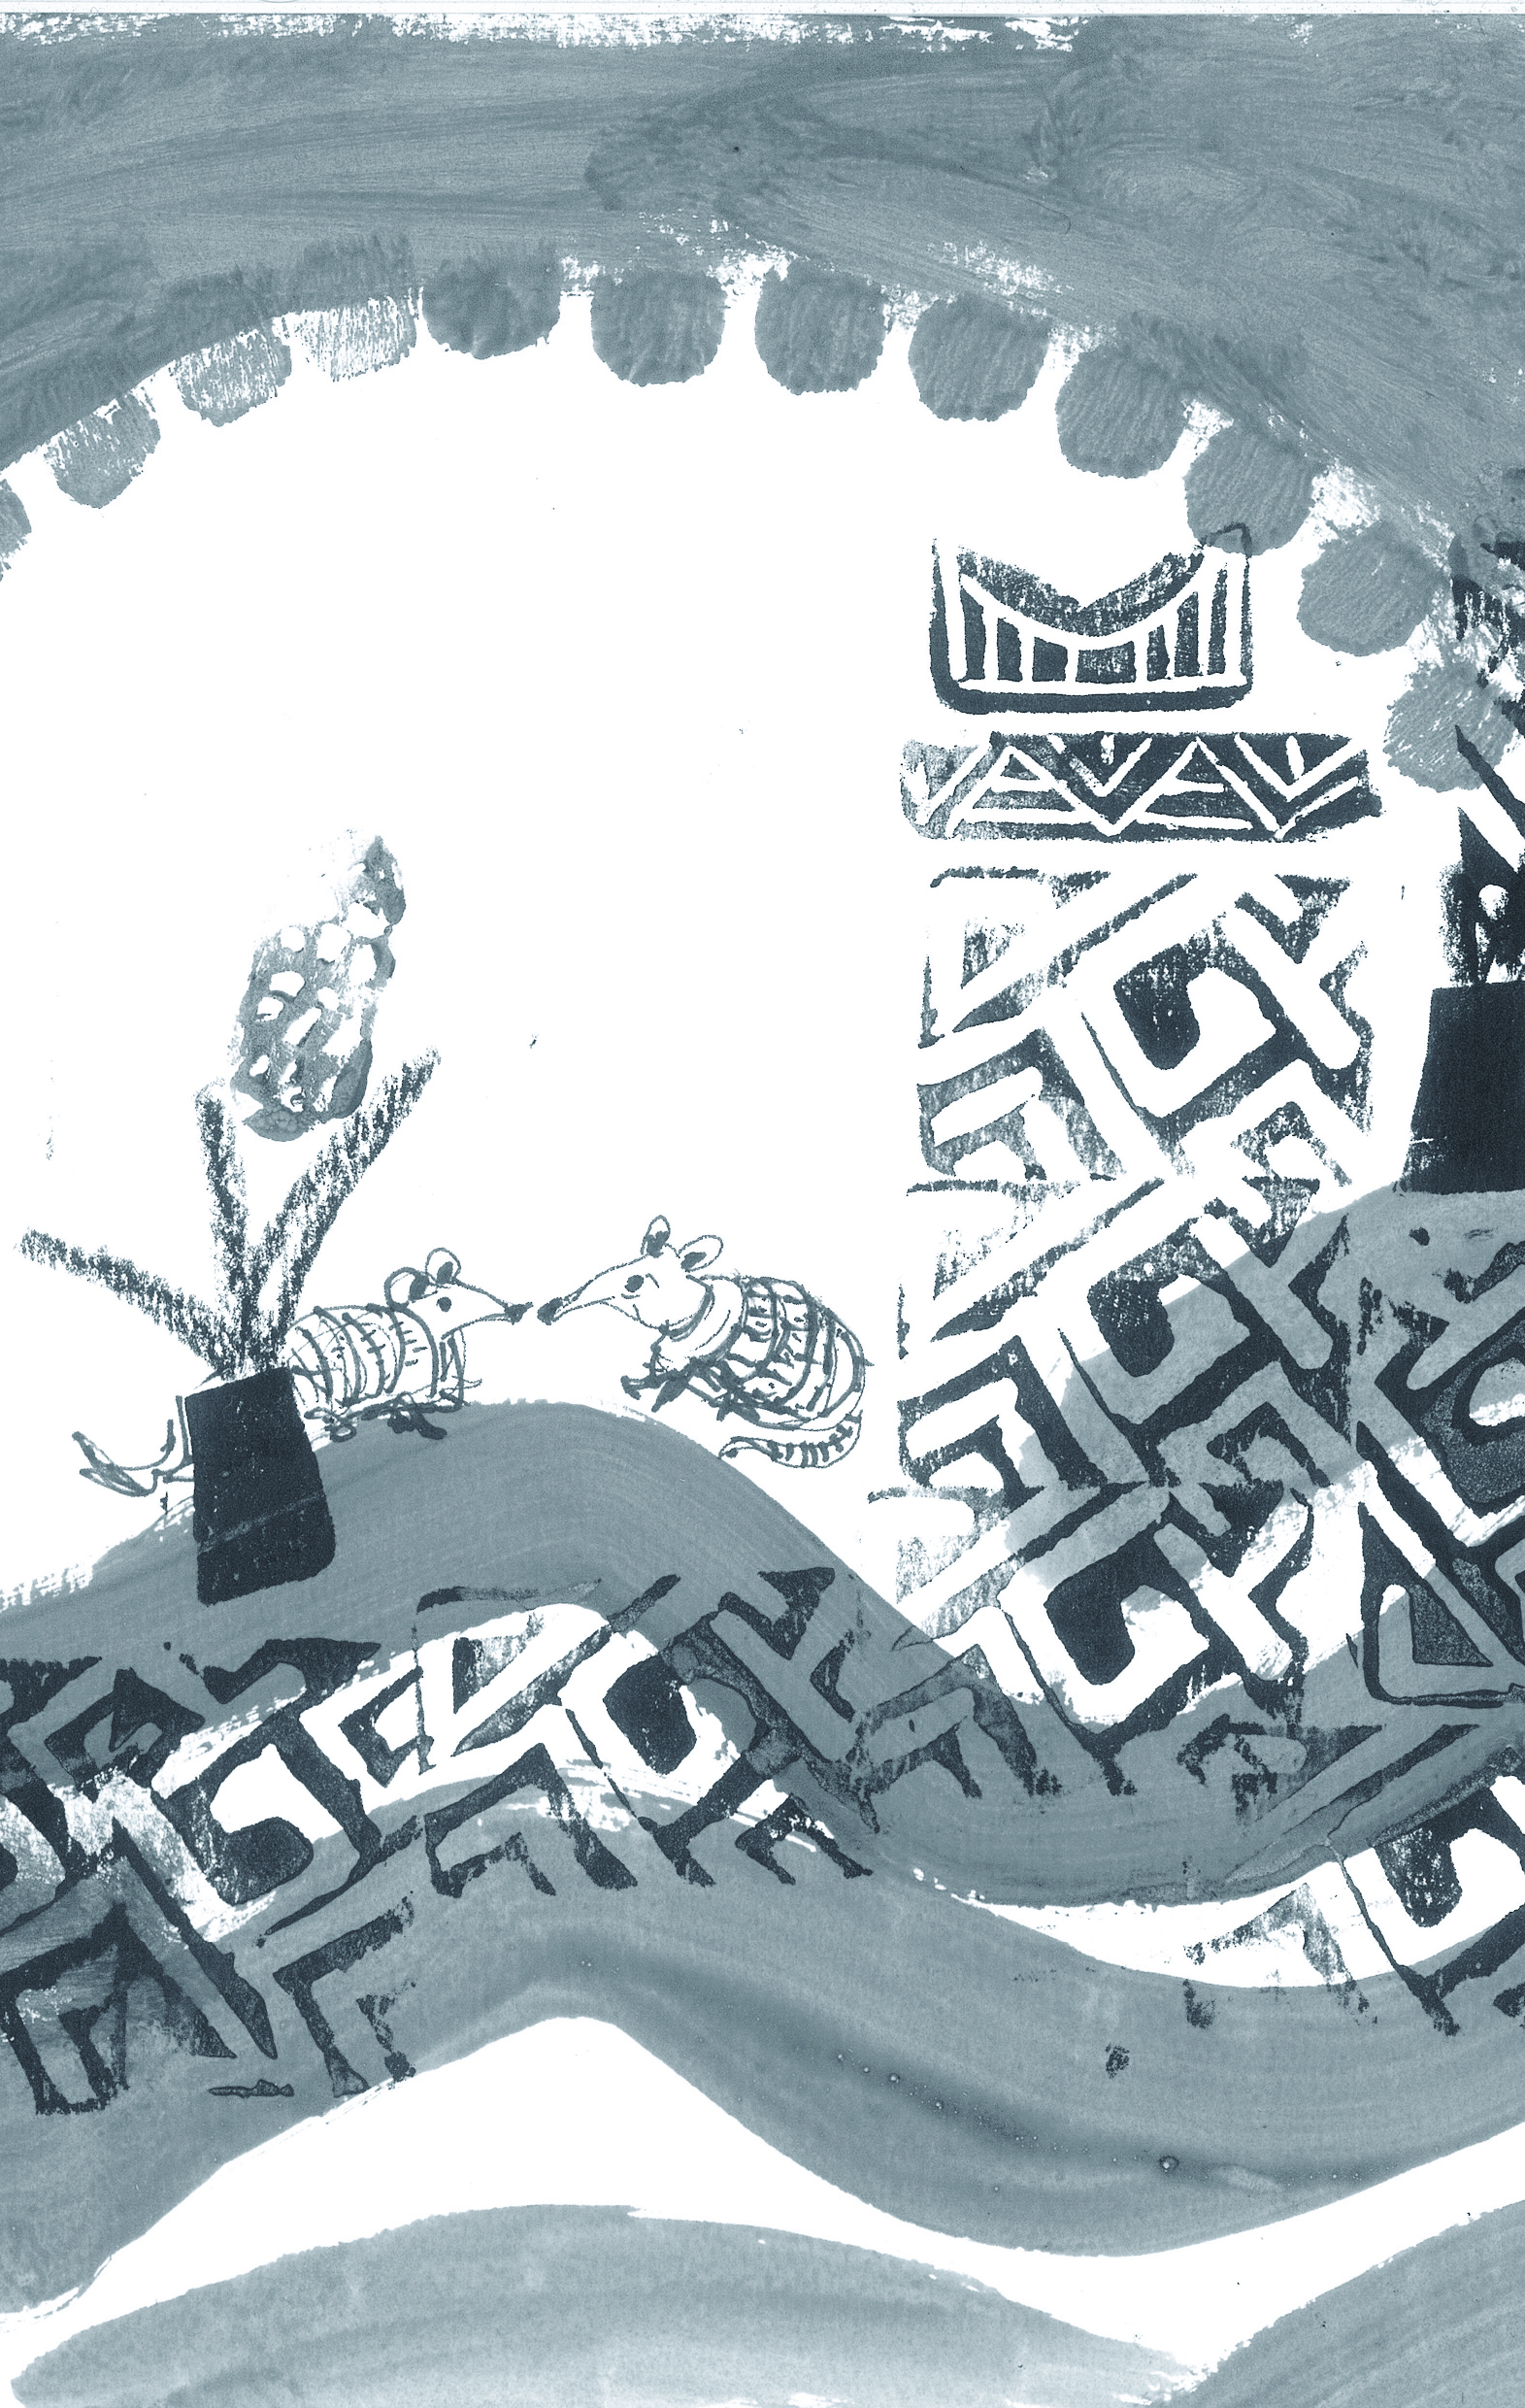
\includegraphics[width=150mm]{./imgs/img12.pdf}
\end{figure}

\chapter*{}

\mbox{}\vspace*{\fill}

% \begin{verse}
% A história diz que quem\\
% domesticou a batata doce para\\
% podermos comer foi o tatu, e\\
% quando não tinha batata doce\\
% para comer, o tatu comia minhoca.\\
% Foi assim que a velha fez para\\
% virar tatu, transformou o corpo\\
% e passou a comer batata doce e,\\
% quando não tinha, comia minhoca.
% \end{verse}

% \begin{verse}
% \textit{Kadi bikindan, yaixin bini kiaki.\\
% Kadimakendan yaixdan\\
% xena besti pimis kiaki.\\
% Yuxabudan eskani kiaki, yaix\\
% katsidan. Hatixunki, yamaki}
% \end{verse}

\letra{A}{história} diz que quem
domesticou a batata doce para
podermos comer foi o tatu, e
quando não tinha batata doce
para comer, o tatu comia minhoca.
Foi assim que a velha fez para
virar tatu, transformou o corpo
e passou a comer batata doce e,
quando não tinha, comia minhoca.

\vspace{2em}

\letra{K}{adi} bikindan, yaixin bini kiaki.
Kadimakendan yaixdan
xena besti pimis kiaki.
Yuxabudan eskani kiaki, yaix
katsidan. Hatixunki, yamaki.

\vspace*{\fill}

\pagebreak
\thispagestyle{empty}
\begin{figure}[H]
\vspace*{-.5cm}
\hspace*{-2.2cm}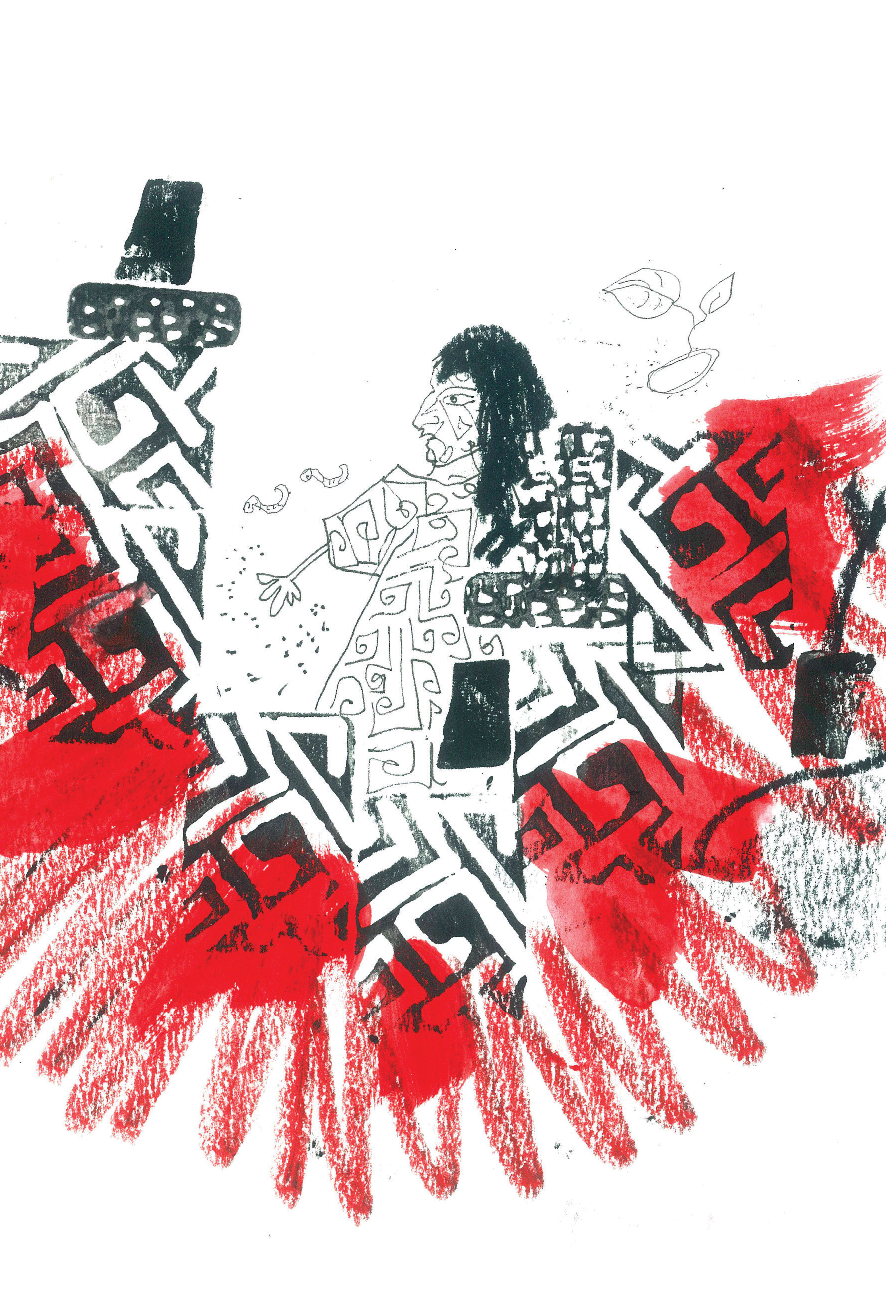
\includegraphics[width=138mm]{./imgs/img13.pdf}
\end{figure}

\endgroup




\pagebreak
\blankpage
%\blankAteven
\pagestyle{empty}
\begingroup
\fontsize{7}{8}\selectfont

{\large\textsc{coleção «hedra edições»}}

\begin{enumerate}
\setlength\parskip{4.2pt}
\setlength\itemsep{-1.4mm}
%\item \textit{Poemas da cabana montanhesa}, Saigy\=o
\item \textit{A arte da guerra}, Maquiavel
\item \textit{A conjuração de Catilina}, Salústio
\item \textit{A cruzada das crianças/ Vidas imaginárias}, Marcel Schwob
\item \textit{A filosofia na era trágica dos gregos}, Friedrich Nietzsche
\item \textit{A fábrica de robôs}, Karel Tchápek 
\item \textit{A história trágica do Doutor Fausto}, Christopher Marlowe
\item \textit{A metamorfose}, Franz Kafka
\item \textit{A monadologia e outros textos}, Gottfried Leibniz
\item \textit{A morte de Ivan Ilitch}, Lev Tolstói 
\item \textit{A velha Izerguil e outros contos}, Maksim Górki
\item \textit{A vida é sonho}, Calderón de la Barca
\item \textit{A volta do parafuso}, Henry James
\item \textit{A voz dos botequins e outros poemas}, Paul Verlaine 
\item \textit{A vênus das peles}, Leopold von Sacher{}-Masoch
\item \textit{A última folha e outros contos}, O.\,Henry
\item \textit{Americanismo e fordismo}, Antonio Gramsci
\item \textit{Anarquia pela educação}, Élisée Reclus 
\item \textit{Apologia de Galileu}, Tommaso Campanella 
\item \textit{Arcana C\oe lestia} e \textit{Apocalipsis revelata}, Emanuel Swedenborg
\item \textit{As bacantes}, Eurípides
\item \textit{Autobiografia de uma pulga}, [Stanislas de Rhodes]
\item \textit{Ação direta e outros escritos}, Voltairine de Cleyre
\item \textit{Balada dos enforcados e outros poemas}, François Villon
\item \textit{Carmilla, a vampira de Karnstein}, Sheridan Le Fanu
\item \textit{Carta sobre a tolerância}, John Locke
\item \textit{Contos clássicos de vampiro}, L.\,Byron, B.\,Stoker \& outros
\item \textit{Contos de amor, de loucura e de morte}, Horacio Quiroga
\item \textit{Contos indianos}, Stéphane Mallarmé
\item \textit{Cultura estética e liberdade}, Friedrich von Schiller
\item \textit{Cântico dos cânticos}, [Salomão]
\item \textit{Dao De Jing}, Lao Zi
\item \textit{Discursos ímpios}, Marquês de Sade
\item \textit{Dissertação sobre as paixões}, David Hume
\item \textit{Diário de um escritor (1873)}, Fiódor Dostoiévski
\item \textit{Diário parisiense e outros escritos}, Walter Benjamin
\item \textit{Diários de Adão e Eva}, Mark Twain
\item \textit{Don Juan}, Molière
\item \textit{Dos novos sistemas na arte}, Kazimir Maliévitch
\item \textit{Educação e sociologia}, Émile Durkheim
\item \textit{Édipo Rei}, Sófocles
\item \textit{Elogio da loucura}, Erasmo de Rotterdam
\item \textit{Émile e Sophie ou os solitários}, Jean-Jacques Rousseau 
\item \textit{Emília Galotti}, Gotthold Ephraim Lessing
\item \textit{Entre camponeses}, Errico Malatesta
\item \textit{Ernestine ou o nascimento do amor}, Stendhal
\item \textit{Escritos revolucionários}, Errico Malatesta
\item \textit{Escritos sobre arte}, Charles Baudelaire
\item \textit{Escritos sobre literatura}, Sigmund Freud
\item \textit{Eu acuso!}, Zola/\,\textit{O processo do capitão Dreyfus}, Rui Barbosa
\item \textit{Explosão: romance da etnologia}, Hubert Fichte
\item \textit{Fedro}, Platão
\item \textit{Feitiço de amor e outros contos}, Ludwig Tieck
\item \textit{Flossie, a Vênus de quinze anos}, [Swinburne]
\item \textit{Fábula de Polifemo e Galateia e outros poemas}, Góngora
\item \textit{Fé e saber}, Georg W.\,F.\,Hegel
\item \textit{Gente de Hemsö}, August Strindberg 
\item \textit{Hawthorne e seus musgos}, Melville
\item \textit{Hino a Afrodite e outros poemas}, Safo de Lesbos 
\item \textit{História da anarquia (vol.\,\textsc{ii})}, Max Nettlau
\item \textit{História da anarquia (vol.\,\textsc{i})}, Max Nettlau
\item \textit{Imitação de Cristo}, Tomás de Kempis
\item \textit{Incidentes da vida de uma escrava}, Harriet Jacobs
\item \textit{Inferno}, August Strindberg
\item \textit{Investigação sobre o entendimento humano}, David Hume
\item \textit{Jazz rural}, Mário de Andrade
\item \textit{Jerusalém}, William Blake
\item \textit{Joana d'Arc}, Jules Michelet
\item \textit{Lira gregra}, Giuliana Ragusa (org.)
\item \textit{Lisístrata}, Aristófanes 
\item \textit{Ludwig Feuerbach e o fim da filosofia clássica alemã}, Friederich Engels
\item \textit{Manifesto comunista}, Karl Marx e Friederich Engels
\item \textit{Memórias do subsolo}, Fiódor Dostoiévski
\item \textit{Metamorfoses}, Ovídio
\item \textit{Micromegas e outros contos}, Voltaire
\item \textit{Narrativa de William W.\,Brown, escravo fugitivo}, William Wells Brown
\item \textit{Nascidos na escravidão: depoimentos norte-americanos}, \textsc{wpa}
\item \textit{No coração das trevas}, Joseph Conrad
\item \textit{Noites egípcias e outros contos}, Aleksandr Púchkin
\item \textit{O casamento do Céu e do Inferno}, William Blake
\item \textit{O cego e outros contos}, \textsc{d.\,h}.\,Lawrence
\item \textit{O chamado de Cthulhu}, \textsc{h.\,p.}\,lovecraft
\item \textit{O contador de histórias e outros textos}, Walter Benjamin
\item \textit{O corno de si próprio e outros contos}, Marquês de Sade
\item \textit{O destino do erudito}, Johann Fichte
\item \textit{O estranho caso do dr.\,Jekyll e Mr. Hyde}, Robert Louis Stevenson
\item \textit{O fim do ciúme e outros contos}, Marcel Proust
\item \textit{O indivíduo, a sociedade e o Estado, e outros ensaios}, Emma Goldman
\item \textit{O ladrão honesto e outros contos}, Fiódor Dostoiévski
\item \textit{O livro de Monelle}, Marcel Schwob
\item \textit{O mundo ou tratado da luz}, René Descartes
\item \textit{O novo Epicuro: as delícias do sexo}, Edward Sellon
\item \textit{O pequeno Zacarias, chamado Cinábrio}, \textsc{e.\,t.\,a.}\,Hoffmann
\item \textit{O primeiro Hamlet}, William Shakespeare
\item \textit{O princípio anarquista e outros ensaios}, Piotr Kropotkin
\item \textit{O princípio do Estado e outros ensaios}, Mikhail Bakunin
\item \textit{O príncipe}, Maquiavel
\item \textit{O que eu vi, o que nós veremos}, Santos-Dumont
\item \textit{O retrato de Dorian Gray}, Oscar Wilde
\item \textit{O sobrinho de Rameau}, Diderot
\item \textit{Ode ao Vento Oeste e outros poemas}, \textsc{p.\,b.}\,Shelley
\item \textit{Ode sobre a melancolia e outros poemas}, John Keats
\item \textit{Odisseia}, Homero
\item \textit{Oliver Twist}, Charles Dickens
\item \textit{Origem do drama barroco}, Walter Benjamin
\item \textit{Os sofrimentos do jovem Werther}, Goethe
\item \textit{Os sovietes traídos pelos bolcheviques}, Rudolf Rocker
\item \textit{Para serem lidas à noite}, Ion Minulescu
\item \textit{Pensamento político de Maquiavel}, Johann Fichte
\item \textit{Pequeno-burgueses}, Maksim Górki
\item \textit{Pequenos poemas em prosa}, Charles Baudelaire
\item \textit{Perversão: a forma erótica do ódio}, Robert Stoller
\item \textit{Poemas}, Lord Byron
\item \textit{Poesia basca: das origens à Guerra Civil} 
\item \textit{Poesia catalã: das origens à Guerra Civil} 
\item \textit{Poesia espanhola: das origens à Guerra Civil} 
\item \textit{Poesia galega: das origens à Guerra Civil} 
\item \textit{Pr\ae terita}, John Ruskin
\item \textit{Primeiro livro dos Amores}, Ovídio
\item \textit{Rashômon e outros contos}, Ryūnosuke Akutagawa
\item \textit{Revolução e liberdade: cartas de 1845 a 1875}, Mikhail Bakunin
\item \textit{Robinson Crusoé}, Daniel Defoe
\item \textit{Romanceiro cigano}, Federico García Lorca
\item \textit{Sagas}, August Strindberg
\item \textit{Sobre a amizade e outros diálogos}, Jorge Luis Borges e Osvaldo Ferrari
\item \textit{Sobre a filosofia e outros diálogos}, Jorge Luis Borges e Osvaldo Ferrari
\item \textit{Sobre a filosofia e seu método (Parerga e paralipomena)} (v.\textsc{ii}, t.\textsc{i}), Arthur Schopenhauer 
\item \textit{Sobre a liberdade}, Stuart Mill
\item \textit{Sobre a utilidade e a desvantagem da histório para a vida}, Friedrich Nietzsche
\item \textit{Sobre a ética (Parerga e paralipomena)} (v.\textsc{ii}, t.\textsc{ii}), Arthur Schopenhauer 
\item \textit{Sobre anarquismo, sexo e casamento}, Emma Goldman
\item \textit{Sobre o riso e a loucura}, [Hipócrates]
\item \textit{Sobre os sonhos e outros diálogos}, Jorge Luis Borges e Osvaldo Ferrari
\item \textit{Sobre verdade e mentira}, Friedrich Nietzsche
\item \textit{Sonetos}, William Shakespeare
\item \textit{Sátiras, fábulas, aforismos e profecias}, Leonardo da Vinci
\item \textit{Teleny, ou o reverso da medalha}, Oscar Wilde
\item \textit{Teogonia}, Hesíodo
\item \textit{Trabalhos e dias}, Hesíodo
\item \textit{Triunfos}, Petrarca
\item \textit{Um anarquista e outros contos}, Joseph Conrad
\item \textit{Viagem aos Estados Unidos}, Alexis de Tocqueville
\item \textit{Viagem em volta do meu quarto}, Xavier de Maistre 
\item \textit{Viagem sentimental}, Laurence Sterne
\end{enumerate}

{\large\textsc{coleção «metabiblioteca»}}

\begin{enumerate}
\setlength\parskip{4.2pt}
\setlength\itemsep{-1.4mm}
\item \textit{A carteira de meu tio}, Joaquim Manuel de Macedo
\item \textit{A cidade e as serras}, Eça de Queirós
\item \textit{A escrava}, Maria Firmina dos Reis
\item \textit{A família Medeiros}, Júlia Lopes de Almeida 
\item \textit{A pele do lobo e outras peças}, Artur Azevedo
\item \textit{Auto da barca do Inferno}, Gil Vicente
\item \textit{Bom Crioulo}, Adolfo Caminha
\item \textit{Cartas a favor da escravidão}, José de Alencar
\item \textit{Contos e novelas}, Júlia Lopes de Almeida
\item \textit{Crime}, Luiz Gama
\item \textit{Democracia}, Luiz Gama
\item \textit{Direito}, Luiz Gama
\item \textit{Elixir do pajé: poemas de humor, sátira e escatologia}, Bernardo Guimarães
\item \textit{Eu}, Augusto dos Anjos
\item \textit{Farsa de Inês Pereira}, Gil Vicente
\item \textit{Helianto}, Orides Fontela
\item \textit{História da província Santa Cruz}, Gandavo
\item \textit{Iracema}, José de Alencar
\item \textit{Liberdade}, Luiz Gama
\item \textit{Mensagem}, Fernando Pessoa
\item \textit{Nós, os sul-americanos}, Flávio de Carvalho
\item \textit{O Ateneu}, Raul Pompeia
\item \textit{O cortiço}, Aluísio Azevedo
\item \textit{O desertor}, Silva Alvarenga
\item \textit{Oração aos moços}, Rui Barbosa
\item \textit{Pai contra mãe e outros contos}, Machado de Assis
\item \textit{Poemas completos de Alberto Caeiro}, Fernando Pessoa
\item \textit{Teatro de êxtase}, Fernando Pessoa
\item \textit{Transposição}, Orides Fontela
\item \textit{Tratado descritivo do Brasil em 1587}, Gabriel Soares de Sousa
\item \textit{Tratados da terra e gente do Brasil}, Fernão Cardim 
\item \textit{Utopia Brasil}, Darcy Ribeiro
\item \textit{Índice das coisas mais notáveis}, Antônio Vieira
\end{enumerate}

\medskip
{\large\textsc{coleção «que horas são?»}}

\begin{enumerate}
\setlength\parskip{4.2pt}
\setlength\itemsep{-1.4mm}
\item \textit{8/1: A rebelião dos manés}, Pedro Fiori Arantes, Fernando Frias e Maria Luiza Meneses
\item \textit{A linguagem fascista}, Carlos Piovezani \& Emilio Gentile
\item \textit{A sociedade de controle}, J.\,Souza; R.\,Avelino; S.\,Amadeu (orgs.)
\item \textit{Ativismo digital hoje}, R.\,Segurado; C.\,Penteado; S.\,Amadeu (orgs.)
\item \textit{Crédito à morte}, Anselm Jappe
\item \textit{Descobrindo o Islã no Brasil}, Karla Lima
\item \textit{Desinformação e democracia}, Rosemary Segurado
\item \textit{Dilma Rousseff e o ódio político}, Tales Ab'Sáber
\item \textit{Labirintos do fascismo} (v.\textsc{iii}), João Bernardo
\item \textit{Labirintos do fascismo} (v.\textsc{ii}), João Bernardo
\item \textit{Labirintos do fascismo} (v.\textsc{iv}), João Bernardo
\item \textit{Labirintos do fascismo} (v.\textsc{i}), João Bernardo
\item \textit{Labirintos do fascismo} (v.\textsc{vi}), João Bernardo
\item \textit{Labirintos do fascismo} (v.\textsc{v}), João Bernardo
\item \textit{Lugar de negro, lugar de branco?}, Douglas Rodrigues Barros
\item \textit{Lulismo, carisma pop e cultura anticrítica}, Tales Ab'Sáber
\item \textit{Machismo, racismo, capitalismo identitário}, Pablo Polese
\item \textit{Michel Temer e o fascismo comum}, Tales Ab'Sáber
\item \textit{O quarto poder: uma outra história}, Paulo Henrique Amorim
\item \textit{Universidade, cidade e cidadania}, Franklin Leopoldo e Silva
\end{enumerate}

\medskip
{\large\textsc{coleção «mundo indígena»}}

\begin{enumerate}
\setlength\parskip{4.2pt}
\setlength\itemsep{-1.4mm}
\item \textit{A folha divina}, Timóteo Verá Tupã Popygua
\item \textit{A mulher que virou tatu}, Eliane Camargo
\item \textit{A terra uma só}, Timóteo Verá Tupã Popygua
\item \textit{A árvore dos cantos}, Pajés Parahiteri
\item \textit{Cantos dos animais primordiais}, Ava Ñomoandyja Atanásio Teixeira
\item \textit{Crônicas de caça e criação}, Uirá Garcia
\item \textit{Círculos de coca e fumaça}, Danilo Paiva Ramos
\item \textit{Folhas divinas}, Timóteo Verá Tupã Popygua
\item \textit{Nas redes guarani}, Valéria Macedo \& Dominique Tilkin-Gallois
\item \textit{Não havia mais homens}, Luciana Storto
\item \textit{O surgimento da noite}, Pajés Parahiteri
\item \textit{O surgimento dos pássaros}, Pajés Parahiteri
\item \textit{Os Aruaques}, Max Schmidt
\item \textit{Os cantos do homem-sombra}, Patience Epps e Danilo Paiva Ramos
\item \textit{Os comedores de terra}, Pajés Parahiteri
\item \textit{Xamanismos ameríndios}, A.\,Barcelos Neto, L.\,Pérez Gil \& D.\,Paiva Ramos
\end{enumerate}

\medskip
{\large\textsc{coleção «ecopolítica»}}

\begin{enumerate}
\setlength\parskip{4.2pt}
\setlength\itemsep{-1.4mm}
\item \textit{Anarquistas na América do Sul}, E.\,Passetti, S.\,Gallo; A.\,Augusto  (orgs.)
\item \textit{Ecopolítica}, E.\,Passetti; A.\,Augusto; B.\,Carneiro; S.\,Oliveira, T.\,Rodrigues  (orgs.)
\item \textit{Pandemia e anarquia}, E.\,Passetti; J.\,da Mata; J.\,Ferreira  (orgs.)
\end{enumerate}

% \medskip
% {\large\textsc{coleção <<anarc>>}}

% \begin{enumerate}
% \setlength\parskip{4.2pt}
% \setlength\itemsep{-1.4mm}
% \item \textit{Anarquia pela educação}, Élisée Reclus 
% \item \textit{Ação direta e outros escritos}, Voltairine de Cleyre
% \item \textit{Entre camponeses}, Errico Malatesta
% \item \textit{Escritos revolucionários}, Errico Malatesta
% \item \textit{História da anarquia (vol.\,\textsc{ii})}, Max Nettlau
% \item \textit{História da anarquia (vol.\,\textsc{i})}, Max Nettlau
% \item \textit{O indivíduo, a sociedade e o Estado, e outros ensaios}, Emma Goldman
% \item \textit{O princípio anarquista e outros ensaios}, Piotr Kropotkin
% \item \textit{O princípio do Estado e outros ensaios}, Mikhail Bakunin
% \item \textit{Os sovietes traídos pelos bolcheviques}, Rudolf Rocker
% \item \textit{Revolução e liberdade: cartas de 1845 a 1875}, Mikhail Bakunin
% \item \textit{Sobre anarquismo, sexo e casamento}, Emma Goldman
% \end{enumerate}

% \medskip
% {\large\textsc{coleção <<narrativas da escravidão>>}}

% \begin{enumerate}
% \setlength\parskip{4.2pt}
% \setlength\itemsep{-1.4mm}
% \item \textit{Incidentes da vida de uma escrava}, Harriet Jacobs
% \item \textit{Narrativa de William W.\,Brown, escravo fugitivo}, William Wells Brown
% \item \textit{Nascidos na escravidão: depoimentos norte-americanos}, \textsc{wpa}
% \end{enumerate}

\pagebreak
\pagebreak

\ifodd\thepage\blankpage\fi

\parindent=0pt
\footnotesize\thispagestyle{empty}

% \noindent\textbf{Dados Internacionais de Catalogação na Publicação -- CIP}\\
% \noindent\textbf{(Câmara Brasileira do Livro, SP, Brasil)}\\

% \dotfill\\

% \hspace{20pt}ISBN 978-65-86238-31-0 (Livro do Estudante)

% \hspace{20pt}ISBN 978-65-86238-30-3 (Manual do Professor)\\[6pt]

% \hspace{20pt}\parbox{190pt}{1. Crônicas Brasileira. 2. Contos Brasileiro. 3. Rosa, Alexandre. I. Título.}\\[6pt]

% \hspace{188pt}\textsc{cdd}-B869.8

% \dotfill

% \noindent{}Elaborado por Regina Célia Paiva da Silva CRB -- 1051\\

\mbox{}\vfill
\begin{center}
		\begin{minipage}{.7\textwidth}\tiny\noindent{}
		\centering\tiny
		Adverte-se aos curiosos que se imprimiu este livro na data de \today, em papel Pólen Soft 80, composto em tipologia Minion Pro, em 11 pontos, com diversos sofwares livres,
		dentre eles Lua\LaTeX e git.\\ 
		\ifdef{\RevisionInfo{}}{\par(v.\,\RevisionInfo)}{}\medskip\\\
		\adforn{64}
		\end{minipage}
\end{center}

%\input{SOL}
%\input{GOKYP}
%\input{LUA}
%\input{OTI}
%\input{RITUAL}
%\input{OSIIP}
%\input{ENCONTRO1}
%\input{ENCONTRO2}
%\input{BIOS}
